\documentclass[11pt]{memoir}

% ——————— PAGE & TYPEBLOCK LAYOUT ———————
\setstocksize{8.5in}{5.5in}
\settrimmedsize{\stockheight}{\stockwidth}{*}
\setlrmarginsandblock{0.75in}{0.5in}{*}
\setulmarginsandblock{0.75in}{0.75in}{*}
\checkandfixthelayout

% ——————— FONTS & MICROTYPOGRAPHY ———————
\usepackage[USenglish]{babel}
\usepackage[autostyle, english=american]{csquotes}
\usepackage{microtype}
\usepackage{fontspec}
\setmainfont{EBGaramond}[
    Path = "font/EBGaramond/",
    Extension = .ttf,
    UprightFont = EBGaramond-Regular,
    BoldFont = EBGaramond-Bold,
    ItalicFont = EBGaramond-Italic,
    BoldItalicFont = EBGaramond-BoldItalic,
    FontFace = {m}{n}{EBGaramond-Medium},
    FontFace = {m}{it}{EBGaramond-MediumItalic},
    FontFace = {sb}{n}{EBGaramond-SemiBold},
    FontFace = {sb}{it}{EBGaramond-SemiBoldItalic},
    FontFace = {eb}{n}{EBGaramond-ExtraBold},
    FontFace = {eb}{it}{EBGaramond-ExtraBoldItalic},
]

% ——————— PARAGRAPH & LINE SETTINGS ———————
\clubpenalty=10000
\widowpenalty=10000

% —————— CHAPTER & SECTION STYLE ——————
\chapterstyle{dash}

\setsecheadstyle{\scshape\centering}
\setsubsecheadstyle{\scshape\centering}
\setsubsubsecheadstyle{\scshape\centering}

% —————— PAGE STYLE & SETUP ——————
\makeoddfoot{plain}{}{}{\thepage}
\makepagestyle{style}
\makeoddhead{style}{\scshape William Blake and the Mysticisms of Sense and Non-Sense}{}{}
\makeevenhead{style}{}{}{\scshape William Blake and the Mysticisms of Sense and Non-Sense}
\makeoddfoot{style}{}{}{\thepage}
\makeevenfoot{style}{\thepage}{}{}
\pagestyle{style}

\renewcommand{\thechapter}{\Roman{chapter}}
\renewcommand{\thesection}{\Roman{section}}

\makeatletter
\let\@afterindentfalse\@afterindenttrue
\@afterindenttrue
\makeatother

\renewcommand{\thepage}{%
    \ifnum\value{page}<7
    \else
        \number\numexpr\value{page}-6\relax
    \fi
}

\setlength{\topskip}{0pt}

\usepackage{perpage}
\MakePerPage[2]{footnote}

\usepackage[splitrule]{footmisc}

\setlength{\skip\footins}{1.5\baselineskip}

\renewcommand{\thefootnote}{\fnsymbol{footnote}}

\usepackage{pdfpages}

\setlength{\afterchapskip}{1.5\baselineskip}

\setaftersecskip{0.5\baselineskip}
\setaftersubsecskip{0.5\baselineskip}

\abnormalparskip{1ex plus 0.5ex minus 0.25ex}

% —————— HYPERREF OPTIONS ——————
\usepackage{hyperref}
\hypersetup{
  hidelinks
}

% —————— TABLE OF CONTENTS OPTIONS ——————
\renewcommand*{\cftchapterfont}{\normalfont}
\renewcommand*{\cftchapterpagefont}{\normalfont}

\renewcommand{\cftdotsep}{1}

\setcounter{tocdepth}{3}

\cftsetindents{subsection}{4\cftsectionindent}{0pt}

% —————— BIBLIOGRAPHY OPTIONS ——————
\usepackage[
  style=numeric,
  refsegment=chapter,
  defernumbers=true,
  sorting=none
]{biblatex}

\DeclareBibliographyCategory{cited}
\AtEveryCitekey{\addtocategory{cited}{\thefield{entrykey}}}

\addbibresource{frontback/bibliography.bib}

\DeclareCiteCommand{\supercite}[\mkbibsuperscript]
  {\usebibmacro{citeindex}%
  \bibopenbracket}
  {\usebibmacro{cite}}
  {\supercitedelim}
  {\bibclosebracket}

% —————— CUSTOM COMMANDS ——————
\usepackage{adjustbox}
\usepackage{tikz}
\usepackage{xparse}
\usepackage{varwidth}

\makeatletter
\newcommand{\quotebox}[2][2em]{%
  \par
  \medskip
  \begingroup
  \centering
  \begin{adjustbox}{}%
    \adjustbox{center,minipage=0.9\linewidth,gstore totalheight=\@tempdima}{\setlength{\parindent}{17pt}#2}%
    \adjustbox{rlap,raise=\dimexpr 0.5\@tempdima - #1 \relax,scale={-1}{-1}}{\Huge``}%
    \hspace{-\linewidth}%
    \adjustbox{rlap,raise=0.5\@tempdima-1.5em,left=\linewidth}{\Huge``}%
  \end{adjustbox}%
  \par
  \medskip
  \endgroup
}
\makeatother

\NewDocumentCommand{\poembox}{O{2em} m}{%
    \begingroup
    \medskip
    \centering
    \begin{tikzpicture}
        \node[inner sep=0pt, anchor=south west] (poem) at (0,0) {\begin{varwidth}{\linewidth}\raggedright #2\end{varwidth}};
        \node[anchor=south east] at ([yshift=\dimexpr-2em+1ex]poem.north west) {\Huge``};
        \node[anchor=north west] at ([yshift=#1]poem.south east) {\scalebox{-1}[-1]{\Huge``}};
    \end{tikzpicture}%
    \par
    \medskip
    \endgroup
}

\newcommand{\blankpage}[1][1]{%
    \newcount\pagecount%
    \pagecount=#1%
    \loop%
        \ifnum\pagecount > 0%
            \clearpage%
            \thispagestyle{empty}%
            \null%
            \clearpage
            \advance\pagecount by -1%
    \repeat%
}

% —————— MAIN DOCUMENT ——————
\begin{document}
  \nocite{*}
  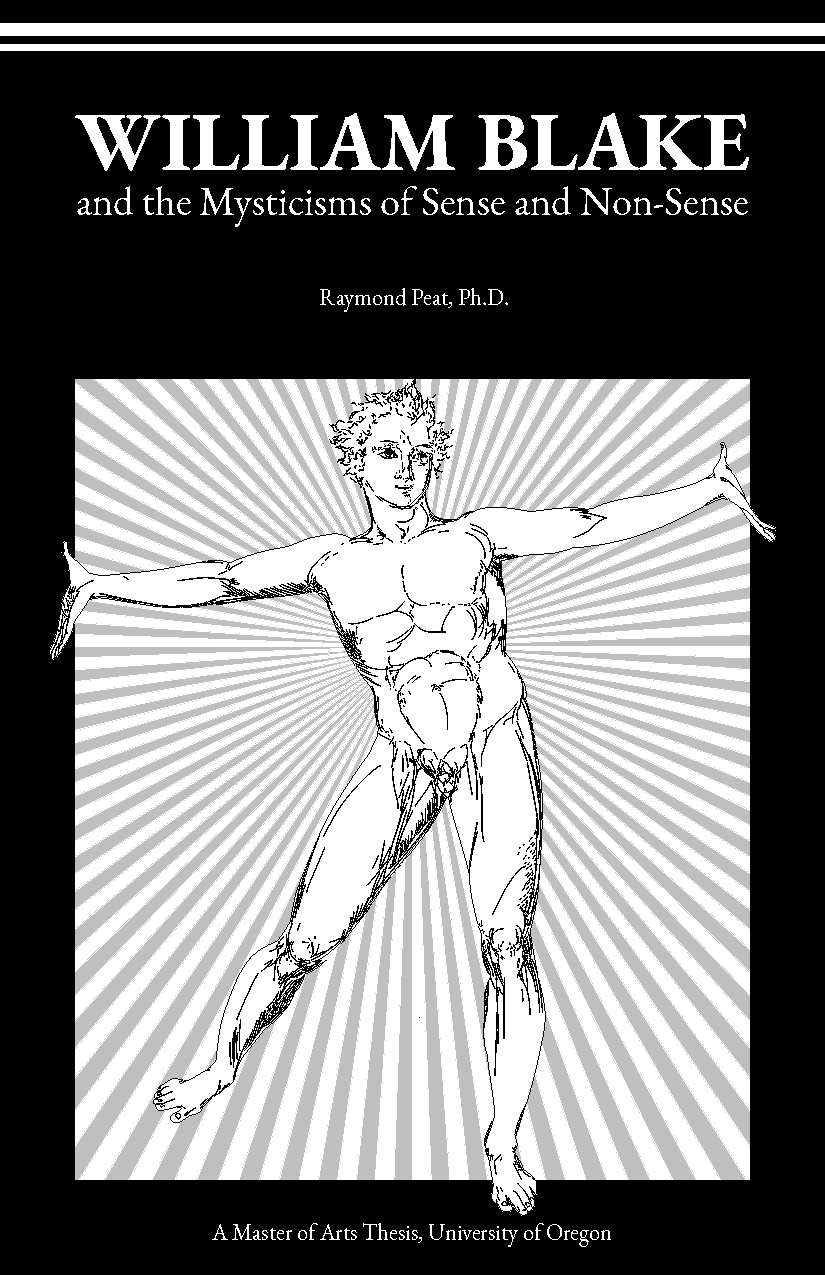
\includepdf[
    pages=1,
    pagecommand={\thispagestyle{empty}},
    fitpaper=true
  ]{frontback/front-cover.pdf}
  \blankpage
  \thispagestyle{empty}

{

    \raggedleft

    Raymond Peat, Ph.D.

    \bigskip
    \bigskip

    {

        \Huge%
        William Blake

        \large%
        and the Mysticisms of Sense and Non-Sense
    
    }

    \bigskip
    \bigskip

    A Thesis; \ June, 1960

}
  \blankpage
  \phantomsection
\pdfbookmark[0]{\contentsname}{toc}

\vspace*{-4\baselineskip}

\tableofcontents*
  \blankpage
  \chapter{History and Definition of Mysticism}

\section{Early Rites and Etymons}

\subsection{Primitive History and Etymology}

Philippe De Felice, in \emph{Poisons Sacrés. Ivresses Divines},
wrote, concerning the immemorial connection between certain
forms of intoxication and religion, that \enquote{The practices
studied in this volume can be observed in every region of
the Earth, among primitives no less than among those who
have reached a high pitch of civilization. We are, therefore,
dealing not with exceptional facts\dots, but with a general
and, in the widest sense of the word, a human phenomenon, the
kind of phenomenon which cannot be disregarded by anyone who
is trying to discover what religion is, and what are the
deep needs which it must satisfy.} Also, the \emph{Encyclopedia
of Philosophy and Religion} includes a discussion of the
primitive religious forms of mana, shamanism, fetishism, and
the traces of medicine men, in which intoxication generally
plays a large part, in its discussion of mysticism.\footnote{\enquote{Most forms of shamanism come within the sphere of mysticism.}\supercite{hastings:philosophy-religion}}
Although many mystics, like Blake, seem to have been \enquote{drunk with
intellectual vision,} rather than with drugs, this association
of drunkenness with \enquote{divine experience} seems to be universal,
except among those extreme dualists, or both the East and the
West, who reject consciousness entirely, and in such cases as
these it is only by their claims, and the claims of their
scholars, that they can be considered mystics:\footnote{Besides the well known shamanistic rites of Siberia, \enquote{divine mushrooms} are known to be used in Borneo, New Guinea, and Mexico, and, at least according to tradition, in China, Japan, and India.\supercite{deropp:drugs-mind, wasson:magic-mushroom} \enquote{\dots there is good reason to assume the existence of a sacred-mushroom cult in Ancient Egypt.}\supercite{puharich:sacred-mushroom}}
the implication is, of course, that \enquote{mysticism} is in some way innately
connected with \enquote{intoxication.} R. Gordon Wasson has written
that there is evidence which links the Greek word \emph{μύσται} with
the root \emph{myoo}, fungus: that fungi, especially mushrooms, are
used as intoxicants is widely known to anthropologists.
It is known, regardless of what explanation, if any, is
given, that natural and related languages contain startling
similarities to European languages; for example, the root
\emph{teo} as used, for instance, in the name of the sacred mushroom,
\emph{teonanacatl}, \enquote{God's flesh,} is obviously similar to the Greek
\emph{Theos} and the Latin \emph{Deus}. Although it cannot be claimed to
be more than an extreme coincidence, a member of the tribe
which uses the sacred mushroom is called a \emph{Mixtec}, which, when
pronounced in Nahuatl, is \emph{identical} in sound to the English
word \enquote{mystic.}

\subsection{Greek Parallels to the Primitive Rites}

Support for Wasson's theory is found in the \enquote{Song to
Demeter} in the \emph{Homeric Hymns},\supercite{hesiod:homeric-hymns}
where Rhea says to Demeter (\emph{μήτηρ} means \enquote{mother,} so Demeter probably represents
\enquote{Mother Earth}): \enquote{\enquote*{But come, my child, obey, and be not
too angry unrelentingly with the dark-clouded son of Conos;
but rather increase forthwith for men the fruit that gives
them life.} So spoke Rhea, and rich-crowned Demeter did
not refuse but straightway made fruit to spring up from the
rich lands.} Although this could, of course, refer to mere
vegetable nourishment, the lines immediately following these
seem to make it clear that it was some sort of vegetable
intoxicant that was gathered by the initiates on their over-night
trip to the countryside, and that was carried back in
a box, from which it would be taken by each initiate:\footnote{\enquote{\dots I have taken (the things) from the sacred chest, having tasted thereof\dots}\supercite{britannica:encyclopedia}}
\enquote{Then she went, and to the kings who deal justice, Triptolemus
and Diocles, the horse-driver, and to doughty Eumolpus and
Celeus, leader of the people, she showed the conduct of the
rites and taught them all her mysteries, to Triptolemus and
Polyxeinus and Diocles also,---awful mysteries which no
one may in any way transgress or pry into or utter, for
deep awe of the gods checks the voice.}\supercite{hesiod:homeric-hymns}
Although \emph{The Encyclopedia of Philosophy and Religion} indicates that, in
Cicero's view, Athens produced \enquote{nothing better than the
mysteries of Eleusis, not only in regard to the ordering and
civilizing of life, but in regard to the furnishing of a good
hope in death,} and that Sophocles believed that \enquote{happiness
in the next world} was confined to \enquote{\dots those who had been
initiated in the mysteries of Eleusis, that is, probably
so far as their fellow-citizens were concerned.}\supercite{hastings:philosophy-religion}
The \enquote{Song to Demeter} does not explicitly impute a doctrine or \enquote{after-
life} to the mysteries: \enquote{Happy is he among men on Earth who
has seen these mysteries; but he who is uninitiate and who
has no part in them, never has lot of liken good things once
he is dead, down in the darkness and gloom.}\supercite{hesiod:homeric-hymns}
This statement, it seems, could be interpreted to represent either a denial
of after-life for those who are not initiated, with no
reference to the future of the initiate, or a statement that
the initiate will have a superior after-life.

\section{Oriental Rites}

\subsection{Hinduism}

The doctrine of the after-life was highly developed in
Greece, regardless of whether a particular \enquote{mystery} contained
the idea, and Pythagoras, or rather Pythagoreans, with
their ideas of the \enquote{wheel of birth} and the transmigration of souls\supercite{britannica:encyclopedia}
(both of which involved the idea of karma, however
it was expressed) seem to have been representative of this
doctrine, as classical Hinduism, with the same particular
ideas, was representative of that doctrine in India. Although
little seems to be known about the actual practices
of \enquote{purification} of the Pythagorean Brotherhood, they can
be considered mystical, by the same criteria which allow
the \emph{Encyclopedia of Philosophy and Religion} to assert that
\enquote{In Hinduism, indeed, in nearly all of its manifestations,
in its most philosophical flights as well as when it
approaches pure shamanism and magic, there are to be found
indications of the mystical temper of mind.}\supercite{hastings:philosophy-religion}\footnote{See also pp. \pageref{self:01} of this thesis a similar statement concerning the classification of Buddhism.}

Although Hinduism is widely considered to be an ascetic religion, 
the \emph{Bhagavad-Gītā} contains what seems to be an
early doctrinal justification for the \enquote{modernized} forms of
the religion, which were modified by the influence of the
primitive Naga and Yaksa worship and the competition of
liberalized Buddhism. The \emph{Gītā} says that some \emph{Yogis} offer
their soul to the \enquote{sacrificial fire} of Brahman, and others
renounce possessions, activity, and sense-perception; however,
immortality and the reaching of \enquote{eternal Brahman,}
besides happiness \enquote{in this world,} can also be obtained by
those who \enquote{allow their minds and senses to wander unchecked,
and try to see Brahman within all exterior sense-objects.
For these, sound and the other sense-objects are the offering,
and sense-enjoyment the sacrificial fire.}\supercite{vyasa:bhagavad-gita}

\phantomsection
\label{self:17}

\subsection{Mature Mahayana Buddhism}

Since the classical Hindu tradition of renunciation is both very well
known and practically identical with the main Christian
mystical tradition, and since the Tantric Hindu movement
closely parallels the \enquote{liberal} Buddhist practices, differing
mainly in its attempt to \enquote{\dots assimilate and adjust itself to
the Orthodox tradition (rather) than to exclude and refute it.}\supercite{heinrich:philosophies-india}
It will be assumed that the discussions of the mature
Mahayana Buddhism and the Catholic Christian mystical tradition
will illustrate the two main types of mysticism sufficiently.

\phantomsection
\label{self:01}

The fact that Buddhism has a greater reputation for being
monistic rather than Hinduism is revealed by the statement in the
\emph{Encyclopedia of the Social Sciences} that Buddhism has spread
into areas which had previously been Christian, Taoist,
Zoroastrian, and even Brahmnist because of its practical
nature, its goals being primarily humanitarian, and psychology
being the means used to achieve them. According to the definition
given by the above, Buddhism can be considered to be
\enquote{mystical} if it makes use of such practices as \enquote{ecstasy,}
\enquote{trance,} and \enquote{consciousness of the absolute,} so it can be
seen that both of these statements about Buddhism can be
simultaneously correct of the mentioned \enquote{practices} are
understood in a monistic sense, and if \enquote{humanitarian} is
not defined too narrowly. The monistic Buddhist might say
that \enquote{through certain trances or exercises man can, in
accordance with the Four Noble Truths,\footnote{(1) The truth of pain, (2) The truth of the cause of pain, (3) The truth of cessation of pain, and (4) The truth of the way that leads to the cessation of pain.\supercite{noss:mans-religions}}
overcome ignorance, and thereby become aware of the highest truth and experience
the highest delight, Maha-Sukha.} The person who desires to
\enquote{overcome his ignorance,} that is, to be initiated, need
only, as in the parallel Hindu and Greek religions, be
\enquote{\dots intelligent,\dots one who abstains from injuring any being,
ever doing good to all, pure, \dots and a nondualist\dots,}\supercite{heinrich:philosophies-india}
That is, women and slaves were not excluded, and could even
become \emph{Gurus}, or teachers of the religion.

The \enquote{metaphysical} explanation of this aspect of Buddhism
is given by Zimmer as follows:

\quotebox{%
    \dots pure compassion is of the essence of the Bodhisattva
    and is  identical with his right perception of the void;
    or, as one might say, it is the primary reflex of the void.\supercite{heinrich:philosophies-india}
    \dots \enquote{The Bodhisattva attains omniscience.}\supercite{heinrich:philosophies-india}\footnotemark
    \ Within the hearts of all creatures compassion is present
    as the sign of their potential Bodhisattvahood; for all things
    are Sunyata, the void---and the pure reflex of this void (which
    is their essential being) is compassion. Compassion (\emph{Karuna})
    indeed is the forge that holds things in manifestation---just
    as it withholds the Bodhisattva from Nirvana.
}

\footnotetext{%
    It is important to note that \emph{all} of those who hold an entirely
    monistic mystical doctrine maintain that \enquote{omniscience} is characteristic
    of the person who has attained the condition of \enquote{inspired perception} or
    \enquote{four-fold vision}: examples are the Mixtec Indians, the Hindus, the Buddhists
    being discussed here, and Blake, who said \enquote{less than all cannot satisfy man.}\supercite{keynes:william-blake}
}

This \enquote{Nirvana} from which the Bodhisattva is withheld by his
compassion refers to the Nirvana of the dualistic mystics,
that is, the ineffable and utterly transcendent reality; the
condition being described above may also be called \enquote{Nirvana,}
but it might be more accurate to limit its name to that used
by the parallel Hindu sects, viz., \enquote{\emph{Mahanirvana}.}\supercite{heinrich:philosophies-india}
Zimmer continued his explanation of monistic Buddhism with an indication
of its contrast to Christianity, Vedantism, and Hinayana
Buddhism, as follows:

\quotebox[2.25em]{%
    \dots this world-supporting condescension of the Bodhisattva\dots in
    spirit and practice\dots takes us one step further (than
    the Christian mystery of the incarnation), since it calls for
    \emph{an unqualified affirmation of \enquote{ignorance}} (Avidya) \emph{as in
    essence identical with \enquote{enlightenment}} (body)---which renders
    archaic the ancient Sankhya-Vedanta-Hinayana modes of Monkism
    rejection or acceptance\dots \enquote{ignorance} (Avidya) is still\dots the
    cause of suffering\dots the benighting affliction of those
    who live in desire and fear, in hope, despair, disgust, and
    sorrow. But the one whose mind is cleansed, whose \enquote{soul,}
    whose selfhood, has become annihilate in the void, he is identical\dots
    mingled with the compassion of the Bodhisattva is a quality,
    therefore, of \enquote{great delight} (Maha-Sukha)\dots hence the
    Bodhisattva wanders everywhere, boundless, fearless, like a lion,\footnotemark
    roaring the lion-roar of Bodhisattva, these three worlds have been
    created, as it were, for---by---and of---the enjoyment of this
    immortal: they are his \emph{Lila}, his \enquote{play.}
}

\footnotetext{See page \pageref{self:02} of this thesis.}

\phantomsection
\label{self:27}

\quotebox[2.25em]{%
    Since the candidate for such knowledge must behave like
    one who has already attained, a programmatic, sacramental
    breaking of the bounds that normally stand as the limits of
    virtue was carefully undertaken in certain schools of the
    Mahayana. In spite of all the scandal that has been spread
    concerning this phase of Buddhist worship, the majority of
    the sacramental breaches (in a society hedged on every side
    by the most meticulous taboos) were not such as would give
    the slightest pause to the usual modern Christian gentleman or lady.
    They consisted in partaking of such forbidden
    foods as fish, meat, spicy dishes, and wines,
    and engaging in sexual intercourse. The sole novelty was that these acts
    were to be undertaken\dots under the direction of a religious
    teacher, being regarded as concomitants of\dots (an) absolutely
    indispensable spiritual exercise.\supercite{heinrich:philosophies-india}\footnotemark
}

\footnotetext{Note especially the comments of Esteson and Wilson in chapter II, besides Blake's statements, for example, pp. \pageref{self:03} of this thesis. D. H. Lawrence has used the same idea, for instance, in \emph{The First Lady Chatterley}: \enquote{\dots inside nature there is a spark which sometimes flies into consciousness\dots as a result of the perfect contact} of opposites.\supercite{lawrence:first-lady-chatterly}}

\phantomsection
\label{self:18}

Elaborating further on the \enquote{metaphysical implications
of the corporeal spirituality} of the rite which has been
stigmatized by the psychologist J. H. Leuba as \enquote{the sexual
indulgences connected with the worship of certain non-civilized
and half-civilized peoples.}\supercite{leuba:god-or-man}
Zimmer says, \enquote{The basic Indian doctrine---the doctrine of transcendental monism,
which merges opposite principles in timeless union---finds no
more striking symbolization anywhere than in the lamasery
cult of the icon of the holy bliss (\emph{Mahāsukha}) of the
united couple.}\supercite{heinrich:philosophies-india}\footnote{It is widely believed\supercite{cheney:walked-with-god} that many of Blake's paintings (as well as books), were destroyed for their \enquote{immorality} (and \enquote{blasphemy}); it is possible that among these were mystical illustrations on the order of the Hindu sculpture of this period, for instance those at Khajuraho.}

\subsection{Taoism}

The preceding suggests, to the typical Western person,
the Taoist doctrine of the \enquote{Ying and Yang,} or \enquote{Yab-Yum,} that
is, the universal creative interplay of opposites;\footnote{Called \enquote{contraries} by Blake, as well as by the Taoists.}
although there was considerable contact between Taoism and Buddhism
during the first six centuries A.D., during which time Taoism
adopted many things from Buddhism, the Yab-Yum doctrine
seems to have originated independently in each place, though
probably earliest in China. A concise summary of the general
doctrine of philosophical Taoism, as well as an indication
of its historical classification, is given by the \emph{Encyclopedia
Britannica} as follows:

\quotebox[2.25em]{%
		The Taoists were mystics, but they were practical
		mystics, and hoped to realize the best social order through
		a harmonious relationship with the Tao. Their idea was
		\enquote{this worldly.} Their mysticism had three stages: (1) the
		purgation, casting out selfishness and self-seeking; (2)
		union with the Tao, by which the individual lost his individuality
		with the distraction of the contraries; (3) power,
		which enabled the individual merged with the Tao to escape
		the limitations of time and space.\supercite{britannica:encyclopedia}
}

Although this summary is worded in the standard Western \enquote{mystical}
terms, implying a conception of mysticism as necessitating
a metaphysic of ultimate dualism, its first two sentences
clearly indicate the intended sense of the \enquote{purgation,}
\enquote{individuality,} and \enquote{escape of time and space}; the material
immediately following reveals the \enquote{standard} Western position.\footnote{See pp. \pageref{self:04}-\pageref{self:05} of this thesis.}

\phantomsection
\label{self:04}

\section{Western Dualism (Christian)}

\subsection{Saints and Semi-Saints, or Emanations and Immanence}

According to the \emph{Encyclopedia of Philosophy and Religion},
the main ideas of Christian mysticism, both Catholic and
Protestant, are that \enquote{behind the visible, material, eternal universe,
which is the \emph{mother} of the one that we see,} and that it is
man's highest goal to apprehend that universe in some supernatural
fashion.\supercite{hastings:philosophy-religion}
In accordance with their dualism, the
Catholic mystics (Boehme will be shown to be typical of a
less dualistic\footnote{It must be noted that the doctrines of \enquote{Emanation} and \enquote{Immanence} are both dualistic philosophies, although the latter does approach monism to some degree. The dualistic distinction is maintained in the doctrine of Immanence by holding that it is \enquote{Being} which is \enquote{Immanent} within \enquote{Becoming.} Dante and St. Thomas Aquinas can be considered representatives of \enquote{Emanation} doctrine, while Plotinus and Boehme support the doctrine of \enquote{Emanation.}\supercite{underhill:mysticism}}
group, mainly Protestants), to some degree\supercite{underhill:mysticism}\footnote{See pp. \pageref{self:06} of this thesis.}
consider the apprehension of the \enquote{supernal reality} to be
dependent upon their \enquote{discarding} of the physical universe.

That for many Catholic mystics the \enquote{mystical experience}
is considered to be some sort of an approximation of death
is indicated by statements from, for instance, St. Bernard,
Meister Johannes Eckhart, and Dionysius, the Areopagite, and
the Orthodoxly accepted\footnote{As expressed by Evelyn Underhill.}
attitudes concerning events in the lives of, for instances, St. Catherine of Genoa and St. Catherine
of Siena. The simplest statement of the idea is probably
Eckhart's: while speaking to God, who appeared to him as a
naked and lovely boy, he asked where God was to be found, and
received the answer \enquote{in departure from everything worldly.}\supercite{cheney:walked-with-god}

St. Bernard, in a more negative statement, said \enquote{fasting,
praying, keeping watch, undergoing disciplines, wearing hair
shirts, sleeping on boards, etc., were all invented because
there is continual opposition of the flesh to the spirit,
the body threatens to overcome the spirit and there is unending
conflict between them.}\supercite{cheney:walked-with-god}
It seems to be a justifiable supposition that the rejection of consciousness by the mystics
increases proportionately with the degree of dualism of the
world-view; Dionysius, who, according to Cheney, tends to
minimize \enquote{the hole of the indwelling Christ,} said, \enquote{We must be
transported wholly out of ourselves and given unto God.},\supercite{underhill:mysticism}
and \enquote{You should, in the purposive practice of mystic contemplation,
escape the senses and lay aside the guidance of the
intellect \dots escaping alike what is and what is not\dots}\supercite{cheney:walked-with-god}

\subsection{Modern Scholars of Christian Mysticism (Dualistic)}

The extent of Dionysius' dualism is far beyond that of the
common \enquote{being-becoming} dichotomy: not only is all of that
which forms the common denominator of the \enquote{being-becoming}
dichotomy, viz., existence, rejected, but a category of \enquote{non-existence}
is oriented, and it is rejected also; that which
constitutes the mystic's goal is so utterly removed from the
ordinary world that it is unknowable, even by the soul. The
use of negative statements and even paradox is reminiscent
of Lao Tzu's statement, \enquote{He who knows does not speak; he who
speaks does not know. Soften its light, submerge its turmoil---this
is the mystic unity.}\supercite{browne:great-scriptures}
Dionysius, however, is more extreme than the Taoists; for instance, in his statement
\enquote{\dots rise upward
toward union with him who is above all knowing
and all being,}\supercite{cheney:walked-with-god}
ineffability is replaced by unknowability, unless
\enquote{the essential mystical darkness, the cloud of unknowing}
indicates merely the absence of verbal knowledge,
which seems extremely doubtful. It is interesting to note
that both of these negative positions, that which clearly
advocates a monistic following of the \enquote{way,} and that which
urges that the soul leave behind physical existence in its
attempted apprehension of the \enquote{divine darkness,} resemble
each other in the denial of existence in the \enquote{highest} (nothing),
(the Tao, and God, respectively), while it is merely
the proper \enquote{goal} of the mystic in which they apparently
differ; that is, they could be said to have the same metaphysics,
while differing in their ethos.

Underhill indicates that the lives of certain saints
reveal the inverse relationship between physical and spiritual
well-being: \enquote{\dots in cases of St. Catherine of Genoa
and St. Catherine of Siena it would seem that as their health
became feebler and the nervous instability always found in
persons of genius increased, their ecstasies became more
frequent\dots}\supercite{underhill:mysticism}
Underhill also quotes St. Thomas on this subject,
saying: \enquote{St. Thomas proves ecstasies (trances) to be
inevitable\dots \enquote*{The higher our mind is raised to the contemplation
of spiritual things,} he says, \enquote*{The more it is abstracted from sensible things.
(But the final term to which contemplation can possibly arrive is the divine substance.)
Therefore, the mind that sees the divine substance must be
totally divorced from the bodily senses, either by death or
\emph{by some rapture}.}}\supercite{underhill:mysticism}
Cheney, a less dualistic commentator on
the mystics, rather than exaulting the state of trance or
near death as the ultimate form of enlightment, says that
those mystics, exemplified by St. Catherine of Siena, were
extremists, \enquote{\dots given to penance and ecstatic visions and
trances\dots}\supercite{cheney:walked-with-god}

Although it is not entirely approved by the dualistic
writers, a physically produced, and sensuously conscious,
\enquote{ecstasy} is not considered by them to be wholly without
value: it seems that the concept of \enquote{mono-ideism} is related
in their minds to spirituality, since, \enquote{In the mystic, the
idea which fills his life is so great a one---the idea of God---that,
in proportion as it is vivid, real, and intimate, it
inevitably tends to monopolize the field of consciousness}\supercite{underhill:mysticism}
with the result that any experience that seems to be mono-ideistic,
or to result from mono-ideism, is considered to be
\enquote{spiritual} to a degree, regardless of its physical origin
and apparently somewhat sensuous nature, since (by their
logic) to exclude sensations numerically is to approach
the transcendent reality more closely.

Thus Boehme, and those others such as St. Ignatius Lovola
whose \enquote{mental eyes} were opened to a superior understanding
by contemplation of a physical object,\footnote{Underhill considers Blake to be a member of this group of \enquote{imperfectly dualistic} mystics; see pp. \pageref{self:07} of this thesis.}
are considered to be mystics of a moderate state of advancement, since it seems that
they, in the dualists language, overcame sensuous perception
to a degree which enabled them to see the spiritual nature of
reality, although it was somewhat contaminated by the remaining
awareness of particular objects. Boehme reveals the dual
nature of the \enquote{union} as he understood it, in which the
finite entity retains its nature while being \enquote{defied} by the
presence of God, in statements such as the following:
\enquote{\dots if thou art born in God, then there is in thyself (in the
circle of thy life) the whole heart of God undivided}\supercite{underhill:mysticism}
and \enquote{\dots the soul (is) set in the deity; the deity penetrateth
through the soul, and dwelleth in the soul, yet the soul doth
not alter it (from being a soul) but only giveth it the
divine source (or property) of the majesty.}\supercite{underhill:mysticism}
Obviously this is a less dualistic general world-view than that of the
mystics who hold the doctrine of emanations, since matter
and spirit are not held to be in absolute opposition, it is
this tendency toward monism that makes Boehme's conception of
unity insufficiently pure and separate for the dualists,
while it is his failure to philosophically remove the distinction
between body, soul, and God, or the \enquote{oversoul,} that
makes his doctrine not entirely acceptable to the \enquote{monistic
mystic}; nevertheless, many of his mystical statements,
that is, his descriptions of the mystical experience, have
been of great value to many such \enquote{monistic mystics,} an
example of such a statement would be his statement that an
intensely perceived object led him to the ability to see
\enquote{the principles and deepest foundations of things.}\supercite{underhill:mysticism}
It is interesting to note that this idea appears also in the descriptions
of the first mystical experiences of John Fon, and others.

Evelyn Underhill, in \emph{Mysticism}, seems to be one of the
most \enquote{valuable} writers on mysticism, because of the fullness
of her statement of the metaphysic which underlies her interpretation
of the experiences of the various subjects considered.
Although she is very definite in her labelling
of other attitudes as wrong, though the \enquote{other enemy} varies,
she at least treats her subject seriously enough to recognize
that there are alternative possible interpretations of the
meaning of \enquote{mysticism,} the definition of mysticism which
she defends in this book is given in the preface as follows:

\clearpage

\quotebox[2.25em]{%
    Broadly speaking, I understand it to be the expression
    of the innate tendency of the human spirit towards complete
    harmony with the transcendental order; whatever be the theological
    formula under which what order is understood. This
    tendency, in great mystics, gradually captures the whole
    field of consciousness; it dominates their life and, in the
    experience called \enquote{mystic union,} attains its end. Whether
    that end be called the God of Christianity, the World-Soul of
    Pantheism, the absolute of philosophy, the desire to attain it
    and the movement towards it---so long as this is a genuine
    life process and not an intellectual speculation---is the
    proper subject of mysticism.\supercite{underhill:mysticism}
}

This generally Neo-Platonic definition of mysticism, said to
be \enquote{\dots its old meaning\dots the science or art of the spiritual
life}\supercite{underhill:mysticism}
is opposed to such \enquote{abuses} of the word as its use
\enquote{\dots as an excuse for every kind of occultism, for dilute
transcendentalism, vapid symbolism, religious or aesthetic
sentimentality, and bad metaphysics.}\supercite{underhill:mysticism}
Apparently, \enquote{every kind of occultism} is intended to include the oldest use of
the word, i.e., the Greek use of it mentioned at the beginning
of this chapter.

\phantomsection
\label{self:12}

Since the above definition depends upon the meaning
\enquote{spiritual}, Miss Underhill's definition of that must be
shown; it clearly cannot be \enquote{naturalistic} in any sense, since
she has said, in the preface to the twelfth edition, \enquote{Determination---more
and more abandoned by its old friends the physicists---is
no longer the chief enemy to a spiritual interpretation
of life and is required by the experience of the
mystics, it is rather a naturalistic monism, a shallow
doctrine of immanence unbalanced by any adequate sense of
transcendence, which now threatens to re-model theology in
a sense which leaves no room for the noblest and purest
reaches of the spiritual life.}\supercite{underhill:mysticism}
That the above definition was purely in the Neo-Platonic tradition is indicated by
her statement that she has consistently believed \enquote{\dots that
the facts of man's spiritual experience pointed to a limited
dualism; a diagram which found place for his contrasting
apprehension of absolute and contingent, being and becoming,
simultaneous and successive. Further, that these facts
involved the existence in him, too, of a certain doubleness,
a higher and lower, natural and transcendental self\dots}\supercite{underhill:mysticism}
This \enquote{limited dualism} is apparently \enquote{limited} only in the
way that the dualism of Plotinus is limited, viz., it is not
one which says that people are entirely alien to the transcendent
reality, which would obviate the possibility of a
mystical experience, but one which is entirely supernaturalist,
except that in the association of a \enquote{soul} with a body
there is some sort of a graduation of reality. The \enquote{soul,} to
Underhill, is apparently stretched between the \enquote{natural and
transcendental} selves, since it is only the \enquote{apex of the
soul\dots which the mystics have always insisted} to be \enquote{the
instrument of their special experience.}\supercite{underhill:mysticism}
Disregarding the degree to which the dualism is limited, it is worthwhile to
note the way in which Underhill elaborates upon the subject
of dualism in relation to mysticism: \enquote{this reinstatement of
the transcendent, the \enquote*{wholly other,} as \emph{the} religious fact,
is perhaps the most fundamental of the philosophic changes
which have directly affected the study of mysticism.}\supercite{underhill:mysticism}

Closely connected with the transcendence of its (mysticism's)
object, are the following two doctrines: \enquote{First that mysticism\dots can
never be the whole content of\dots religion. It requires
to be embodied in some degree in history, dogma, and
institutions\dots secondly, that the antithesis between the
religions of \enquote*{authority} and \enquote*{spirit,} the \enquote*{church} and
the \enquote*{mystic} is false.}\supercite{underhill:mysticism}
Since nothing in the assumption of a \enquote*{transcendent object} leads necessarily to these doctrines,
it can be assumed at this point that a favorable treatment
will be given to those mystics and remained within the
church. while a less favorable treatment will be
given the less Orthodox individuals. This is clearly indicated
by Miss Underhill's statement that \enquote{The \enquote*{exclusive} mystic,
who condemns all outward forms and rejects the support
of the religious complex, is an abnormality. He inevitably
tends towards Pantheism, and seldom exhibits in its richness
the unitive life.}\supercite{underhill:mysticism}

In explaining the \enquote{characteristics of mysticism} Underhill
gives four \enquote{rules} which can be used to \enquote{test} the
validity of cases which claim \enquote{to rank among the mystics};
they are intended especially to be reputations of two of
William James' \enquote{four harms}\footnote{Those who use the word in what seems to be its \enquote{true,} or earliest meaning, i.e., in its radical signification, would also deny that the experience was ineffable and transient.}
of the mystic state, namely, \enquote{noetic quality} and \enquote{passivity.} The first \enquote{rule} is intended
to distinguish the mystical experience from the
simply mystical philosophy, I.E., Platonism: \enquote{1. True
mysticism is active and practical, not passive and theoretical.}
In developing this idea Underhill emphasized this well-known
distinction between the philosophies of Plato and
Plotinus, viz., that Plato's \enquote{unity} was only an intellectual
thing, an knowledge of the \enquote{truth,} while that of Plotinus
was an experiential thing, a \enquote{flight of the alone to the alone.}\supercite{turnbull:essence-of-plotinus}
Plotinus is said to be one of those (Platonic
philosophers) \enquote{\dots who have passed far beyond the limits of
their own philosophy, and abandoned the making of diagrams
for an experience, however imperfect, of the reality at which
these diagrams hint.}\supercite{underhill:mysticism}
Platonism, says Underhill, \enquote{\dots is the reaction of the intellectualist upon mystical truth}\supercite{underhill:mysticism}
and it is implied that in Plato's case the \enquote{mystic truth} was from
a source other than himself.

The second \enquote{rule} is one which is very important to note
for its implications, concerning ethics, which contrast so
sharply with the statements made by or about the \enquote{mystics} of
the \enquote{naturalistic} sort:

\phantomsection
\label{self:06}

\quotebox[2.25em]{%
    Its (mysticism's) aims are wholly transcendental and
    spiritual. It is in no way concerned with adding to, exploring,
    re-arranging, or improving anything in the visible
    universe. The mystic brushes aside that universe, even in
    its supernormal manifestations.\supercite{underhill:mysticism}
}

The third \enquote{rule} seems to be merely a slight variation
of the first: the changeless \enquote{\dots one is for the mystic, not
merely the reality of all that is, but also a living and
personal object of love; never an object of exploration.}\supercite{underhill:mysticism}

The fourth, however, offers some interesting facts concerning
the \enquote{definite psychological experience} which is entailed
by mysticism: the experience, which is sometimes called
\enquote{ecstasy,} though Underhill prefers the words \enquote{unitive state,}
or the \enquote{mystic life process,} is defined only by its prerequisites,
which are \enquote{the apprehension of God,} \enquote{the passion
for the absolute,} \enquote{an appropraite psychological make-up,}
\enquote{a nature capable of extraordinary concentration, an exalted
moral emotion,} and \enquote{a nervous organization of the artistic type.}\supercite{underhill:mysticism}

Sheldon Cheney, in \emph{Men Who Have Walked with God},\supercite{cheney:walked-with-god}
gives a definition of Christian mysticism which, though it
applies to several famous mystics to some degree, seems to
be determined by a consideration of Blake's mystical life;
it is distinctly not the definition that would be given by
a writer of the type of Evelyn Underhill, although that
type would agree with his statement that Oriental mysticism
is \enquote{negative.} \enquote{The Christian mystic,} Cheney says in defining
the motivation which apparently is for him the explanation
of the \enquote{Blakean} character of Christian mysticism,\footnote{That Cheney is clearly in error when he thus opposes Christian to \enquote{Oriental}---later specified as Buddhist---mysticism is seen when one notes the great stress given by the Buddhists to the \enquote{motivation}---compassion (Karuna)---that \enquote{withholds the Bodhisattva from Nirvana.}\supercite{heinrich:philosophies-india}}
\enquote{while losing nothing of the sublimity of the abstract union with the absolute\footnote{See the footnote on pp. \pageref{self:08} of this thesis; this though a distinctly non-Blakean idea, is consonant with Cheney's interpretation of Blake.}
as known to Eastern sages, is likely to substitute a \enquote*{contemplation of the heart}---Bernard's phrase---for
intellectual meditiation.}\supercite{cheney:walked-with-god}
\enquote{The Christian founders substituted, in place of the abstract one, a sympathetic God-Father.}\supercite{cheney:walked-with-god}

As opposed to the motivation, Cheney describes the
character, or what might be called the \enquote{ethic,} of Christian
mysticism: \enquote{Typically, the Christian mystic curbs the inclination
to seclusion.} \enquote{\dots he follows contemplation with
service, abstention with participation in active works.}\supercite{cheney:walked-with-god}
\enquote{\dots from the first mystics among the Apostles to that latest
Christian mystic poet (Blake) whose hand never rested from
\enquote*{my endeavour to restore the Golden Age,} to restore the age
when man finds \enquote*{Eternity in an hour}---from first to last the
great Christian mystics stayed out their lifetimes in the
current of mortal occupations\dots they have returned\dots to
illumine that corner of the Earth about them, or it may be
a whole nation or realm, with light from their vision and
their understanding.}\supercite{cheney:walked-with-god}

\enquote{\dots Christian mysticism implies less retreat from the
world, a withdrawal into the light of the Divine, than an
enlargement of the mortal horizon and a mission among men to
reveal to them the joy of knowing eternal life in the midst
of mortal affairs.}\supercite{cheney:walked-with-god}
Cheney shows Buddhism to be a religion that induces \enquote{an admirable social ethic, but only as incidental
along a path of personal mystic experience.} He says that
the end of that path is \enquote{\dots Nirvana, or extinction of selfhood
in the ocean of eternal divinity.}\footnote{Etymologically, \enquote{\emph{Nirvana}} can be considered to mean simply \enquote{without the forest,} with, possible, the implication of the colloquial English, \enquote{out of the woods}: \emph{nir}, \enquote{without,} and \emph{vana}, \enquote{the forest.}\supercite{heinrich:philosophies-india}}

\section{Technical Studies of Mysticism}

\subsection{Philosophical}

Cheney continues the discussion of the relation of Buddhism
to Christianity with the somewhat Blakean statement, \enquote{There is a negative aspect to the Buddhist faith, a denial
of the\dots importance of life in the world, which is fundamentally
different from the message that can be read in the words, and
in the life of Jesus.}\supercite{cheney:walked-with-god}
That the difference is mainly one degree is indicated by his summary: \enquote{Nevertheless the
Christian faith advances a way of life not unlike the Buddhist
in\dots its positing of divine immersion or communion as
the highest good in mortal life.}\supercite{cheney:walked-with-god}

It is in accord with the incompleteness of Cheney's
dualism that he is concerned with the mystical experience
as a means to the end of social well-being.\supercite{cheney:walked-with-god}

Alfred Kazin's discussion of Christian mysticism\supercite{kazin:portable-blake}
should be especially valuable to this chapter, since it seems to be
written with at least a fair amount of objectivity, while
Kazin is a very well-known Blakean scholar. Christian mysticism, he says:

\quotebox[2.25em]{%
    \dots is founded on dualism. It is rooted in the belief
    that man is a battleground between the spirit and the flesh,
    between the temptations of Earth and God as the highest God.
    The mystic way is the logical and extreme manifestation of
    the spiritual will, obedient to a faith in supernatural
    authority, to throw off the body and find an ultimate release in
    the Godhead. Christian mysticism is based upon a
    mortification of the body so absolute that it attains a condition
    of ecstasy. To the mystic, God is the nucleus of the
    creation, and man in his Earthly life is a dislodged atom
    that must find its way back. The mystic begins with submission
    to a divine order, which he accepts with such conviction
    that Earthly life becomes nothing to him. He lives
    only for the journey of the soul that will take him away,
    upward to God. What would be physical pain to others, to
    him is purgation.
}

\phantomsection
\label{self:05}

Of course, there are several weaknesses in this sort of
generalization, including the omission of definitions for
such terms as \enquote{ecstasy,} especially with reference to the
different Christian beliefs concerning that doctrine, and
the implication that there is only one, simple, degree of
dualism, besides the necessary neglect of even the most important
Non-Christian mysticisms, but it does serve the important function
of providing a fairly objective, over-all view of the subject
by one who is, apparently, an \enquote{outsider.}

\phantomsection
\label{self:15}

A nineteenth century psychologist, Ernst Mach, in writing
an epistemology for scientists\supercite{boring:experimental-psychology}
(the first chapter of which is called \enquote{Antimetaphysical}), used the \enquote{facts} of the
\enquote{liberal} mystical tradition, viz., elimination of the \enquote{theoretical} self,
but not of the sense-consciousness, affirmation of dreams as
\enquote{valid knowledge,} and denial of the Platonists' \enquote{realm of eternal ideal existences,}
but seems not to have used them as the basis for a \enquote{psychotherapy}
(with a goal of higher, more intense consciousness, rather than
of \enquote{normality}), as the Buddhists, for instance, have done. Edwin G. Boring,\supercite{boring:experimental-psychology}
in explaining Mach's ideas of consciousness and the world, said \enquote{sensations are not observed; they are given. Being given,
they cannot be shown to be in error. Illusions are \enquote*{illusory}: there are none,
or rather, the straight rod thrust into water is sent, and, if there
be any illusion, it is that the rod is still straight. There is no ego;
there are only sensory data. If we say \enquote*{it lightens,} we ought also to say, \enquote*{it thinks};
\emph{cogitat}, not \emph{cogito}. \enquote*{The world consists only of our sensations.}
Dreams are as valid knowledge as perception.}\supercite{boring:experimental-psychology}
All that is eliminated in this denial of the existence of \enquote{ego} is
the abstract conception of consciousness: consciousness is
here considered to be an \enquote{unbounded} system of sensations, and
the tendency to give conscious value to assumptions of
non-temporal existences, either \enquote{outside} (\enquote{the world consists\dots}, etc.),
or \enquote{inside} (\enquote{There is no ego\dots}), is
rejected, and, of course, this includes the Platonic idea
of \enquote{eternal ideal existences} and the dualists' belief in
a soul distinct from the body.\footnote{See chapter III, second section, of this thesis.}

A very different attitude will be discussed next, as a
contrast for the purpose of showing that an opposition exists
between the facts of monistic mysticism and those of dualistic
mysticism; and that this opposition might be based on different
attitudes towards symbols, symbols being \enquote{things} the
peculiar nature of which is ignored, in favor of their
\enquote{meaning,} that is, another \enquote{thing} which is, by a mental
process, associated with the first.

An attempt to define \enquote{mysticism} philosophically has
been made by a well-known contemporary philosopher, Charles
Morris, in an essay called \enquote{Comments on Mysticism and its Language,}\supercite{hayakawa:language-meaning-maturity}
in which he explains his belief that the concept of language---based on
mental interpretation \enquote{\dots is essential to the understanding of art,
myths, magic, the totem, religion, prestige, race prejudice, and the complex types of perception}\supercite{hayakawa:language-meaning-maturity}
as well as mysticism.

Morris' explanation of language as the basis of mysticism
rests upon his idea of \enquote{the role-taking function of language}:
it is his belief that by means of \enquote{\dots language one can symbolize times
and places other than the here and now, and persons and things
other than the speaker himself}\supercite{hayakawa:language-meaning-maturity}
and, in a sense, \enquote{become} the things which are \enquote{signified.} The point
to be stressed, he says, \enquote{\dots is that in this socially derived
process of role-taking one can become symbolically an object
other than the self of the here and now\dots}\supercite{hayakawa:language-meaning-maturity}\footnote{The fallacy of these ideas should be obvious: a thing which \emph{means} \enquote{far away}or \enquote{near by} is a different thing from human conscious existence in a certain location, and even if possession of a symbol were equivalent to possession of the existence represented by the symbol, the quality of subjective consciousness must, by definition, be described (when referring to its location, without \enquote{objectifying} it, or describing it relationally) by the word \enquote{here}; \enquote{note here,} as Morris fails to see, is purely a relational statement, giving the location of an object which is extraneous to the conscious speaker. It can be seen, therefore, that the most extreme modification of consciousness that could be obtained by this method would be the possession of the \enquote{existence represented by the symbol} (which is denied above), the possession of an \enquote{existent} environment made up by the \enquote{existences} \enquote{carried within} the symbols. Of course, if symbols are considered to be transcendently valuable, the shift of consciousness from sensuous reality to a \enquote{world of symbols} might be considered to be sufficiently valuable to deserve the name \enquote{mystic experience.}}
According to his theory, \enquote{\dots this simultaneous, or nearly simultaneous arousal
of the complex and often contradictory role-taking processes made
possible by language constitutes an essential part of the mystical
experience.}\supercite{hayakawa:language-meaning-maturity}

The experience of seeing ordinary objects \enquote{\dots through
symbolic eyes enlarged by cosmic wandering} is \enquote{liberating,}
according to Morris; \enquote{Einstein has testified to this, and has
even spoken of it as \enquote*{the sower of all true art and science.}}
Whether the experience is liberating or not depends upon one's
conception of \enquote{freedom,} but the rest of Morris' statement is
decidedly false: what Einstein spoke of as the \enquote{mystical feeling,} the
\enquote{sower\dots} etc., was simply a non-dogmatic perception of the universe, or reality.
That his attitude was entirely contradictory to that ascribed to him by Morris is indicated
by his own analysis of his mental activity:\supercite{ghiselin:creative-process}
\enquote{The words or the language, as they are written or spoken,
do not seem to play any role in my mechanism of thought.}
\enquote{Conventional words or other signs have to be sought for laboriously only
in a secondary stage\dots} \enquote{In a stage when words intervene at all\dots they intervene only in a secondary stage\dots}\supercite{ghiselin:creative-process}
Morris also claims that \enquote{The psychologist, A. H. Maslow,
has found it (the \enquote*{symbolic experience}) to be present in some degree
in persons of maximum creativity and \enquote*{psychological health,}} and that it is \enquote{\dots available in varying degrees
to all persons, regardless of their scientific and philosophical commitments.}\supercite{hayakawa:language-meaning-maturity}
The truth in this case is that Maslow clearly and explicitly said that the \enquote{mystical} consciousness
appears only in those individuals who have been \enquote{liberated} from the effects of
language and symbols, that the brain-injured and neurotics are typically limited
to \enquote{symbolic} understanding of reality, and that \enquote{philosophical commitments}
are integrally related to the frequency and intensity, and even to the very existence
of the mystical experience. These attitudes will be more fully discussed in the
following section on Maslow, and an alternate form, viz.,
that the \enquote{mystical experience} may have been artificial (or \enquote{chemical}), rather than
an exclusively natural (or \enquote{psychological}) origin, as represented by Aldous Huxley, will then
be discussed, while the relation between \enquote{philosophical commitments} and \enquote{natural sources}
will be considered again in chapter III.

\phantomsection
\label{self:29}

\subsection{Psychological}

A. H. Maslow, a psychologist who has spent much time in the
study of what he considers to be people in an extremely rare condition
of complete psychological health, says that for these subjects, \enquote{Those
subjective expressions that have been called the mystic experience and described so well by
William James are a fairly common experience\dots}\supercite{maslow:motivation-personality}
He says that these experiences are related to the strong, free emotions which
are typical of his subjects. Reminiscent of the famous ideas of
\enquote{mystic marriage} or \enquote{sacred betrothal,}\footnote{See St. Teresa's \enquote{spiritual marriage,}\supercite{underhill:mysticism}}
but with the differences that his subjects are speaking from a point of view
opposite to that of the famous mystics, Maslow says, \enquote{My interest and attention
in this subject (mysticism) was first enlisted by several of my subjects who described their
sexual orgasms in vaguely familiar terms which later I remembered had been used by
various writers to describe what they called the mystic experience.} More specifically,
he says, \enquote{There were the same feelings of limitless horizons opening up to the vision,
the feeling of being simultaneously more powerful and also more helpless than one ever
was before, the feeling of great ecstasy and wonder and awe, the loss of placing
in time and space with, finally, the conviction that something extremely important and
valuable had happened, so that the subject is to some extent transformed and
strengthened even in his daily life by such experience.}\supercite{maslow:motivation-personality}

\clearpage

Revealing himself to be, in general, allied with those
called by Underhill \enquote{monists and philosophic naturalists,}\footnote{E.g., Leuba, who believes that \enquote{life, more life, a larger, richer, more satisfying life, is in the last analysis the end of religion.}\supercite{oxford:the-monist} Colin Wilson's position (see chapter II), is practically identical with this.}
Maslow says, \enquote{It is quite important to dissociate this experience
from any theological or supernatural reference, even
though for thousands of years they have been linked. None
of our subjects spontaneously made any such tie-up.}\supercite{maslow:motivation-personality}
He suggests that renaming it \enquote{the oceanic feeling} (Freud's term for it)
would help to remove any implication of the supernatural from it.

Another attitude toward the mystical experience that seems to be
common among the \enquote{monists}\footnote{See the comments by Huxley on pp. \pageref{self:09}-\pageref{self:10} of this thesis.}
is that it can occur in varying intensities: \enquote{The theological literature has
generally assumed an absolute, qualitive difference between the
mystic experience and all others. As soon as it is divorced from
supernatural reference and studied as a natural phenomenon,
it becomes possible to place the mystic experience
on a quantitative continuum from intense to mild.}\supercite{maslow:motivation-personality}
On the basis of this attitude he indicates that the \enquote{\emph{mild} mystic experience}
occurs in many or even most persons, and that a \enquote{favored individual}
will experience it many times a day.\supercite{maslow:motivation-personality}
The acute mystical experience is, he says, \enquote{\dots a tremendous intensification of \emph{any} experiences in which there
is a loss of self of transcendence of it,}\supercite{maslow:motivation-personality}
for instance, intense sensuous experience. \enquote{It may even be that the so-called mystic experience is the perfect and extreme
expression of\dots full appreciation of all the characteristics of the particular phenomenon.}\supercite{maslow:motivation-personality}

\phantomsection
\label{self:30}

Maslow believes, as Huxley does, that language (and its associated abstraction and associative reasoning)
limits the experiences of the \enquote{oceanic feeling}: \enquote{\dots it is a screen
between reality and the human being.}\supercite{maslow:motivation-personality}
\enquote{It is\dots very obviously and frankly a means\dots for dulling the perceptions\dots}\supercite{maslow:motivation-personality}
To overcome the limiting effects of language and an education which is
concerned mainly with memory (\enquote{far too much occupied with the intellectual analysis}),\supercite{whitehead:modes-of-thought}
Maslow says that it is necessary to be concerned with \enquote{\dots fresh experiences, with concrete and particular realities.}\supercite{maslow:motivation-personality}

As Cheney and Huxley do, Maslow believes that the mystical sort of consciousness
can have tremendous effects on society: he describes a society constituted entirely of
people who resemble his \enquote{subjects} and gives his opinion that it would be the best society possible.
In this society \enquote{\dots the deepest layers of the human nature could show themselves with great ease.}\supercite{maslow:motivation-personality}

Finally, the interrelations of \enquote{intellectual intoxication,}
which, it seems, might also be called \enquote{biological,} \enquote{psychological,}
or \enquote{sensory} intoxication, with certain kinds of chemical intoxication,
and their contrasts to symbolic, dualistic, and \enquote{transcendent} \enquote{mystical
experiences,} will be illustrated by a discussion of the entire
subject by another \enquote{monistic-naturalistic} mystic, Aldous Huxley.

\phantomsection
\label{self:09}

Aldous Huxley, who has shown a Blakean influence in his
writings for several decades (e.g., \emph{The Cicadas, and Other Poems}), gives
in \emph{The Doors of Perception} a description of his
personal chemically induced \enquote{mystical experience,} which, he
is convinced, resembles the experiences of Blake, whose
\enquote{mental species,} he believes, \enquote{\dots is fairly widely distributed
even in the urban-industrial societies of the present day.}\supercite{huxley:doors-of-perception}
Although Huxley believes himself to be a poor subject for the experiment
(which began with the taking of four-tenths of a gram of mescalin, the synthetically produced
form of the drug which is found naturally in the Aztec's plant-god \emph{Peyotl},
and which is biochemically similar to that found in the other
Aztec plant-god, \emph{Teonanacatl}), saying that he had \enquote{always been
a poor visualizer,} and that his mental images \enquote{have little
substance and absolutely no autonomous life of their own,}
the intensity of the experience was apparently sufficient to
cause him to alter some of his theories of religion and metaphysics
toward a more complete agreement with those of Blake.\supercite{huxley:doors-of-perception}

Huxley describes the mystical experience both indirectly
and directly, that is, he limits the field of mysticism by
discrediting dualism, and he describes the experience of
seeing \enquote{infinity} in the world of material objects. Among
his somewhat negative demonstrations of the nature of mysticism
is a comment on Plato:

\quotebox[2.25em]{%
    \dots Plato seems to have made the enormous, the grotesque mistake
    of separating being from becoming and identifying it with
    the mathematical abstraction of the idea. He could never,
    poor fellow, have seen a bunch of flowers shining with their
    own inner light and all but quivering under the pressure of
    the significance with which they were charged; could never
    have perceived that what rose and iris and carnation so
    intensely signified was nothing more, and nothing less,
    than what they were---a transience that was yet eternal life\dots\supercite{huxley:doors-of-perception}
}

Thus Huxley uses a sort of Platonic language to completely
deny Plato's main doctrine, i.e., that there is a higher order
of being which is perfect and unchanging, which was the basis
for most of the subsequent Western philosophy and, therefore,
of Western mysticism until the rise of Western pantheism and
pantheistic mysticism came with such philosophers as Benedict Spinoza.

It is because of his perception of a long tradition of
erroneous philosophy and false mysticism in the West that
Huxley turns, in this book, to the Orient for most of the
examples of historic parallels to his experience. This attitude
is summed up in the statement:

\quotebox[2.25em]{%
    In their art no less than in their religion, the Taoists
    and the Zen Buddhists looked\dots through the Void at \enquote{the ten
    thousand things} of objective reality. Because of their doctrine
    of the Word made flesh, Christians should have been
    able, from the first, to adopt a similar attitude towards
    the universe around them. But because of the doctrine of
    the Fall, they found it very hard to do so. As recently as
    three hundred years ago an expression of thorough-going
    world denial and even world condemnation was both orthodox
    and comprehensible.\supercite{huxley:doors-of-perception}
}

In a more positive mood, Huxley reveals what must be done to achieve
the \enquote{real} mystic consciousness, or, it could be said, what must be done to overcome the
false perception which is associated with a dualistic attitude it is simply
that \enquote{\dots we must preserve and, if necessary, intensify our
ability to look at the world directly and not through that
half opaque medium of concepts, which distorts every given fact into the
all too familiar likeness of some generic label or explanatory abstraction.}\supercite{huxley:doors-of-perception}

\phantomsection
\label{self:10}

Concerning his \enquote{looking at the world directly,} Huxley
says, \enquote{\dots now I know contemplation at its height.}\supercite{huxley:doors-of-perception}
and \enquote{my actual experience had been, was still, of an indefinite
duration or alternatively of a perpetual present\footnotemark
made up of one continually changing apocalypse.}\supercite{huxley:doors-of-perception}
Again, while looking at the flowers (mentioned above in connection with his criticism of Plato)
which shone \enquote{with their own inner light,}
he was conscious of them as \enquote{\dots a bundle of minute, unique particulars\footnotemark
in which\dots was to be seen the divine source of all existence,}\supercite{huxley:doors-of-perception}
and said, concerning \enquote{The Beatific Vision, \emph{Sat Chit Ananda}, Being-Awareness-Bliss,} \enquote{for the first
time I understood, not on the verbal level, not by inchoate hints or
at a distance, but precisely and completely what those
prodigious syllables referred to.}\supercite{huxley:doors-of-perception}
Although some people in approximately the same circumstances will experience extra-sensory
perceptions, and some will \enquote{discover a world of visionary beauty:} (he says, concerning this
fact, \enquote{like mescalin takers, many mystics perceive supernaturally brilliant colors,
not only with the inward eye, but even in the objective world around them.}),\supercite{huxley:doors-of-perception}
the more intense forms of experience as described by him seem to be of the most valuable for an understanding of mysticism. These are, first, the experience
of \enquote{\dots the glory, the infinite value and meaningfulness of naked existence, of the given, unconceptualized events,}\supercite{huxley:doors-of-perception}
and, secondly, \enquote{the final stage,} in which it is known \enquote{that
all is in all---that all is actually each.}
This is as near, I take it, as a finite mind can ever come to \enquote{perceiving everything that is
happening everywhere in the universe.}\supercite{huxley:doors-of-perception}
These two statements seem to imply, respectively monism and a sort of determinism;
the last sentence of that quotation \enquote{\dots a finite mind,} however,
seems to contradict the meaning of the preceding statement
that \enquote{all is in all,} that is, that each thing, is,
truly, infinite in some way. It seems obvious that Huxley is, in
effect, two persons, one who, under the influence of mescalin, can
experience and apparently be convinced of, certain things, and
the other, his ordinary self, who can remember the experiences
of the other self well enough to describe them vividly, but who is not
completely convinced of the meaning contained in them. Although he is aware of
this dual personality (except in an instance such as that
above, which involves the intellectual understanding of the world in
general, and which was revealed in Huxley by an
unintentional self-contradiction) of the mescalin taker,
Huxley is convinced that the chemically induced \enquote{mystical experience} causes
a permanent, and beneficial, change in the ethical beliefs
and functioning of the subject.\supercite{huxley:doors-of-perception}

\footnotetext{Note the striking similarity to Blake's comment, \enquote{a vision of the eternal now}\supercite{keynes:william-blake} concerning Lavater's aphorism: \enquote{whatever is visible is the vessel\dots of the invisible past, present, future---as man penetrates to this more, or perceives it less, he raises or depresses his dignity of being.} See pp. \pageref{self:11} of this thesis.}

\footnotetext{See pp. [illegible] of this thesis.}
  \chapter[Analysis of the Scholarship Which Considers Blake's Mysticism]{Analysis of the Scholarship Which Considers Blake's Mysticism}

\section{Categorization}

The writings which consider Blake as a \enquote{mystic} can be
divided, as \enquote{philosophizing} in general can, into the categories of (1)
emotionally treated discussions of what is
apparently a conventional association between the object
(Blake's works) and the label (\enquote{mystic}), which discussions
offer nothing more than information concerning the author,
(2) mainly rational applications of standard definitions
(either \enquote{colloquial} or \enquote{scholarly}) to the object, which
are valuable only if a highly specific (\enquote{scholarly}) definition
is shown to be positively applicable, since to \enquote{define} an
object by indicating that it is outside a very limited
class is much less accurate than the inexact method of
indicating that it is within a very broad class (the
\enquote{colloquial definition,} which in the case of \enquote{mysticism} is
especially broad because of its confusion with \enquote{mystery,} that
is, anything unfamiliar), and (3) considerations of the
given (perceptual) realities of the object, with the application
of a label which has approximately accurate etymological
implications, and from which all irrelevant meanings have
been eliminated. In general, studies which were published
before 1915 can be included in the first category, since the
study of mysticism seems to have been of a very vague nature
up to that time, and in the second category can be included
those studies which class Blake as a \enquote{mystic,} a \enquote{non-mystic,}
or \enquote{an example of psychic principle} (e.g., \enquote{sublimation}),
either entirely without definition of the term or with a
definition which has no discoverable reference to observable
reality, that is, which is not applicable to Blake.\footnote{It is thus suggested that the Blake studies in the second category are without value, since it is not granted that any \enquote{scholarly} (as opposed to \enquote{colloquial}) definition is \enquote{positively applicable} to Blake's works.}
The fact that the third category is used when the second category
contains the possibility of a satisfactory explanation of Blake
implies that there is no \enquote{standard} definition which
can be applied correctly to Blake's position; only one of this
group uses the word \enquote{mysticism} in describing Blake, and in
that case the word is apparently used in that \enquote{unusual,}
\enquote{functional} rather than supernatural, sense used by the Greek
mysteries and Maslow, and applied to Buddhism and other
socially oriented \enquote{cults.}

\section{First Category}

Since the first group has been designated as \enquote{unrelated,}
it will be sufficient to mention the names of typical authors
and their books, with comments where necessary.

Adaline Butterworth's \emph{William Blake, Mystic}\supercite{butterworth:blake-mystic}
is an ultimate example of irrelevant, though enthusiastic, discourse, supposedly
upon the subject of the title.

Neither Gardner\supercite{gardner:vision-and-vesture}
nor Selincourt\supercite{de-selincourt:william-blake}
reveal what could be considered a substantial grasp of Blake's \enquote{meaning.}

Edwin Ellis, in \emph{The Real Blake},\supercite{ellis:real-blake} expatiates energetically, as
do those mentioned above, mainly in verbose inanities,\footnote{Ellis' rather active mind produced such samples as the following, which elaborates upon the idea of mental activity, or \enquote{this is Christendom}: \enquote{Blake\dots coined a term for it (\enquote*{virtual velocity}) himself. It was mind in a state of patience. He accounted for motion by the idea that wind is eternal, but patience is not. Patience removed, mind moves\dots}}
yet certain of his statements are not entirely without value, for instance: \enquote{\dots to attain\dots inspiration is
the duty of all who can do so\dots} and \enquote{In Heaven all is brotherhood. \enquote*{In eternity all is vision.} There is
a socialism of the soul there, and communism of property.} Supporting analysis, however, is lacking.

The introduction of the Chatto and Windus edition of
\emph{The Marriage of Heaven and Hell}\supercite{blake:heaven-and-hell}
contains the somewhat interesting statement: \enquote{\dots Blake believed that he knew the
secret, and possessed the faculty of obtaining more than a glimpse of the pure light; he believed, too, that
what men call reality is in truth but a dreamland, and that imagination alone \enquote*{in this age} can lead us to the real,} and
the supporting statements that Blake's \enquote{faculty} was \enquote{an extreme development of the
faulty of creative imagination,} and that this \enquote{hypertrophy} \enquote{approaches, in short, a new sense,} which is
\enquote{incomprehensible to the ordinary man.} Despite this apparent analysis, it seems that the above work must
be included with this first group because it makes use of, to support the explanation, the
term \enquote{creative imagination,} which does not have a \enquote{standard} definition (which would
place it in the second category), without giving a definition for it (which would place it in the
third category). Another factor that seems to place this work entirely within
this category is the extremely naive discussion of Blake's supposed \enquote{symbolic Christianity}: without
any substantiation from Blake's writings (which, incidentally, are directly contradictory: see chapter three of this thesis),
it is indicated that the \enquote{central tenets} of his religion are in some way concerned with the interrelations
of \enquote{inspiration} and \enquote{symbols}; although this near-deification of symbols is typical of Freudianism, which
was developing around this time, the only Freudian-religious study of Blake to be considered in this chapter is more
appropriately included in the second category, since the naive attitude toward symbols is hidden by its concern with
the \enquote{cause} of religion, rather than its (supposed) \enquote{goal.}

\section{Second Category}

Julien Green, in \enquote{William Blake, Prophet,}\supercite{green:blake-prophet}
says that Blake was a \enquote{true mystic,} in that he \enquote{separated} the human,
the mere appearances, from the spirit, the eternal aspect, of man:
that is, he was a dualist; however, it seems that the only support given for this belief is some
biographical information which reveals that Blake experienced the extremes of love and hate. Because of the particularization given to the term \enquote{mystic,} and the failure to show a relationship,
even in the significant particulars, and much less in [illegible], this study is excluded from both the first
and third categories, and is therefore to be considered (merely to indicate that it deserves, unlike Butterworth's and Ellis' of
the first, some respect) a member of the second. Approximately the same can be said about Mark Schorer's \enquote{William Blake and
the Cosmic Nadir,}\supercite{schorer:cosmic-nadir}
except that in this article the author's belief that the concept of the \enquote{Fall} (of Man) lies
at the bottom of Blake's whole system is emphasized; this concept seems to be of such integral importance to the following
scholar, Evelyn Underhill, that it requires no particular elaboration.

\clearpage

\phantomsection
\label{self:07}

On the basis of the discussion of Underhill's \enquote{definition} of
mysticism in the first chapter of this thesis, it should
be obvious that her treatment of Blake will not be included in the
third \enquote{category,} since Blake's mysticism constitutes only a small part of her large study, and
seemingly could easily be lightly, and thus inaccurately, treated; however, Underhill's study of
mysticism was sufficiently broad, and her understanding of Blake accurate enough that she, without
warping Blake extremely,\footnote{See pp. \pageref{self:12} of this thesis; also the comment on pp. \pageref{self:13}}
explained his position with some degree of thoroughness, though
the accuracy of the basic explanation can be doubted. It has already been
pointed out\footnotemark[\value{footnote}]
that Underhill, as representative of the Catholic
scholars of mysticism, considers Blake, as well as Boehme, to be a mystic
who is \enquote{imperfectly dualistic}; he is further described as representing a \enquote{stage of growth
which the mystics calls the illuminative way,} which is only the \enquote{first mystic life.}\supercite{underhill:mysticism}
This sort of mystic, probably because of his natural temperament (\enquote{In the artist, the senses have somewhat
hindered the perfect inebriation of the soul}\supercite{underhill:mysticism}), has come to rest, Underhill believes, after an
initial period of \enquote{oscillation} between opposing and embracing the \enquote{intuitions} of the Absolute, during which
period certain \enquote{discordant} characteristics have been eliminated from the personality, and is convinced that he has
attained the \enquote{divine and veritable world} that his understanding is \enquote{final and complete.} he is, however, Underhill
says, \enquote{ignorant as yet of that consummation of love which overpasses the proceedings of the inward eye and
ear\dots and, absorbed in this new blissful act of vision, forgets that it belongs to those who
are still \emph{in via}.}\supercite{underhill:mysticism} Most of the people who reach this stage, apparently
including Blake, fail to go on to the \enquote{Source,}
the \enquote{true goal} which lies far beyond this merely \enquote{illuminated} state.

The preceding analysis of Blake, and similar mystics, by
Underhill is based on a distinction between two types of
\enquote{passive imaginary vision}--by which is meant \enquote{spontaneous mental
pictures at which the self looks, but in the action of which it does not participate---,}\footnote{Blake seems to represent a variation of the above described \enquote{imaginary vision,} since, although there was apparently no sensorial hallucinations, i.e., the self saw sharply and clearly, but \enquote{perfectly aware that it\dots did so in virtue of its most precious organ}---the faculty of imagination, Blake at least claimed to have participated in certain of his visions, as when he shocked aqquatinces by telling them he had just returned from conversation with a fairy, or that, he had touched the sky; if Underhill were familiar with these statements it would probably add to her opinion that many of the experiences of \enquote{such visionaries as Boehme and Blake\dots are far more occult than mystical in character.}\supercite{underhill:mysticism}}
viz., symbolic and personal. Blake is apparently considered to be the \enquote{artistic type} who
experiences \enquote{symbolic vision,} which are the form taken by the
meditations of those \enquote{good visualizers} such as St. Ignatius Loyola (and the students of Raja Yoga),
who advise that a \enquote{deliberate effort} be made to visualize the subject dwelt upon, rather than to attend
to it \enquote{discursively.}\supercite{underhill:mysticism}
The personal form of the \enquote{vision} is considered to be, rather than
that is apparently merely an unusually efficacious form of meditiation, \enquote{a true contact of the soul with
the absolute life\dots,} one of \enquote{\dots those genuine mystic states in which the immanent God, formless, but capable
of assuming all forms, expressed himself in vision\dots}\supercite{underhill:mysticism}

Another form of \enquote{vision} which apparently \enquote{ranks} above the
two types of \enquote{imaginary vision,} namely, \enquote{intellectual vision,} in
which \enquote{Nothing is seen, even with the eyes of the mind\dots}\supercite{underhill:mysticism}
is also, though inconsistently and falsely, attributed by Underhill to Blake: \enquote{\dots all pure mystics\dots have drunk, with Blake, from
that cup of intellectual vision which is the chalice of the spirit of life\dots}\supercite{underhill:mysticism}
This, however, seems to be simply a minor confusion, since nowhere in her many references to Blake does she consider him to be more than merely one of the most
intensely mystical artists. Although in her summary of Blake, she calls him a \enquote{mystical genius}, Underhill undoubtedly believes that
he, as the other \enquote{English Protestant mystics,}\supercite{underhill:mysticism}
was \enquote{an abnormality} and that he failed to exhibit \enquote{in its richness the unitive life.}\supercite{underhill:mysticism}\footnote{See the first chapter of this thesis.}

If Underhill seems to have understood Blake fairly well, and \enquote{disapproved} of him somewhat, in accordance with her
dualistic position, and other dualists discussed earlier seem to have misunderstood him while \enquote{approving} of him, the
following writer, Sheldon Cheney, compromises between these two positions.

Cheney, a unique combination of a Platonic mind, enthusiasm for Blake, and a high degree of consistency in his explanation
of Blake's beliefs, seems to be one of the two most significant Christian commentators on Blake's ideas; the other,
Evelyn Underhill, is the more valuable for a clear definition of Christian mysticism in terms of which Blake is evaluated;
but Cheney seems to reveal the more perfect understanding of Blake: Cheney's \enquote{system} tended
to adapt to Blake, while Underhill seems to have \enquote{adapted} Blake somewhat to Platonic dualism,
for example, Cheney shows his Platonic attitude, without altering Blake too much, when he said that
Blake \enquote{believed that the soul is, during its time-conditioned life on Earth, a wanderer from
the realm of pure spirit, from an Eden that exists eternally\dots,}\supercite{cheney:walked-with-god}
yet when he, in common with Colin Wilson, says, \enquote{he spoke too of the pleasures of sex as a gateway to vision, a holy gateway
opening upon the clearest eternal seeing of which the soul is capable,}\supercite{cheney:walked-with-god}
he seemed to have discarded his Platonism temporarily, since he makes no attempt to adapt that statement to a larger theory; a
writer of Evelyn Underhill's type would have either omitted this reference or would have shown it to be an indication
either of Blake's inconsistency, or of his \enquote{materialism,} the preceding, however, is not a complete indication
of Cheney's application of Platonism to Blake's beliefs: near the end of his chapter on Blake, there is at least one
instance in which he seems to contradict the statement quoted above, namely, \enquote{nothing could be farther from the sensual, wilful Superman
of Nietzsche,}\supercite{cheney:walked-with-god}
referring to \enquote{Man} in Blake's line \enquote{Thou art a Man, God is no more.} This statement, which
contrasts Blake's \enquote{man} to Nietzsche's \enquote{Superman,} is, however, apparently contradicted by nearly two pages of discussion
of the similarities of the differences between Blake's and Nietzsche's ideas of the \enquote{Superman,} this discussion
begins with the statement, \enquote{William Blake was, as certain philosophers have pointed out, a forerunner of Nietzsche's and
of the cult of the exalted individualism.}\supercite{cheney:walked-with-god}
\enquote{Blake,} Cheney says here, \enquote{\dots can be said to go along with them (the Nietzscheans)
brilliantly in his preliminary destructive phase\dots}
The difference between Blake's and Nietzsche's ideas of the\supercite{cheney:walked-with-god}
\enquote{Superman,} Cheney says, is that Blake adds spirituality to the idea of
\enquote{an individual who is a Superman only physically and intellectually.}\supercite{cheney:walked-with-god}

\phantomsection
\label{self:19}

Cheney divides Blake's mystical \enquote{say} into two parts, as follows: \enquote{The only
half of the struggle upward is the cultivation of multifold vision, the training of the faculties
of spiritual seeing, of clairvoyance. There then remains the more purifying, the more holy, half of the
\enquote*{way,} the process that ends with the restoration of oneness within divinity.}\supercite{cheney:walked-with-god}
Since he says that the first part is \enquote{perceiving the divine in everything} is, as he says in this same paragraph, perceiving
that (in Blake's words), \enquote{everything on Earth\dots in its essence is God,} this perception is enough to
realize the \enquote{oneness with divinity,} unless, of course, it is insisted, in the Platonic or dualistic fashion,

\clearpage

\noindent that \enquote{a thing is separate from its essence,}\footnote{It will be noted in chapter three that \enquote{essence} is shown to be seperate from \enquote{things} i.e., from \enquote{everything on Earth,} and that it is used by Blake as an equivalent to \enquote{God} the \enquote{omnipotent, uncreate} (as distinguished from \enquote{infinite} man as \enquote{God}), but the problem which Cheney makes for himself (and fails to solve), by using the characteristically Christian mystical idea of a two (or more) step \enquote{way} and the other Christian and/or Neo-Platonic idea of \enquote{union with (the universal) God,} is avoided, since, to the best of my knowledge, Blake made no comment other than those which indicate that a recognition of the universal God (called by Underhill \enquote{entelechy} and the spirit of \enquote{becoming}) leads to a recognition of man's \enquote{particular,} yet \enquote{infinite} (see pp. \pageref{self:14} of this thesis) and god-like \enquote{identity.}}
and if this is supposed to be the case Cheney neglects to give any explanation of how the gap is to be bridged.

Cheney's general evaluation of Blake as a mystic is wholehearted:\linebreak
\enquote{William Blake \emph{was} the mystic, imagining, visioning,
walking with God.} \enquote{He is the most genuine and most illuminating mystic in the British Line, and not to be
matched in any country in the Western world during his century.}\supercite{cheney:walked-with-god}
\enquote{Blake's unique importance in the history of
prophecy and mysticism is that he expressed with more beauty than any other, in poetry and in paintings, this message of the spirit
(\enquote*{The individual\dots can be lifted up\dots in mortal life, to that realm of divine illumination and experience}), in terms essentially
Christian yet universal.}\supercite{cheney:walked-with-god}

\phantomsection
\label{self:08}

The editors of \emph{The Cambridge History of English Literature}\supercite{cambridge:english-literature}
seem to have had approximately the same attitude toward
Blake as does Cheney, that is, they seem to have been aware of a relation between a concern with ethics and
slightly dualistic mysticism: \enquote{His mystical faith freed him from the barren materialism of his age and opened to him in
vision the world lying beyond the range of physical senses. Hence, the greater warmth of his ethical creed; and his
preoccupation with the supernatural, which he never consciously shaped to literary ends, is yet the source of the peculiar
imaginative quality of his work\dots} Although these peculiar comments are more meaningful than most of the others written
during the same period (before 1915), some of which are considered on the first category of this chapter, they are
typical of that group in their neglect to define \enquote{mystical faith,} and to give support for the statement that Blake was
preoccupied with the \enquote{supernatural.}

Schorer's article, \enquote{Blake as a Religious Poet,} in the \emph{Sewanee Review},\supercite{schorer:blake-poet}
seems to belong to the second category, since a \enquote{standard} definition of mysticism, viz., \enquote{\dots mysticism is the systematic search for
the transcendental absolute, the uncreated God, through the repudiation of worldly claims and
social values\dots}\supercite{schorer:blake-poet}
is used, although it is used only negatively: according to this definition, Schorer
believes that Blake was not in the least \enquote{mystical,} and was not even a \enquote{religious} poet. Except for the way that Schorer chooses
in this article to use the term \enquote{visionary,} rather than a redefined \enquote{mystic,} to distinguish between the two types of
\enquote{mysticism,} this article might be included in the third group, which includes those studies which consider Blake objectively
without disregarding his \enquote{psychological} aspects; the use of \enquote{visionary} here seems to exclude all but the political or
practical aspects of the \enquote{positive mysticisms} outlined in the first chapter. Schorer's main error seems to be a failure
to see a common denominator for the supposedly mutually exclusive areas of society and \enquote{mystical theology.}

\section{Third Category}

Finally, for the second category, a brief statement by the novelist, D. H. Lawrence, is worth
considering, although its only justification for inclusion in this category is its \enquote{negative} attitude toward what is
implied to be a purely negative \enquote{mysticism,} i.e., it rejects the application of either the popular meaning \enquote{mysterious} or the
scholarly meaning \enquote{divorced from life} to \enquote{Blake's} and Lawrence's work, rather
than attempting to elucidate positively Blake's position. It seems to be Lawrence's implication that certain
forces in society habitually attempt to vitiate works of a certain type (by asserting that their purpose is \enquote{other worldly}), apparently
those which are \enquote{revolutionary} attempts to make men more intensely aware of their existence. This statement was made concerning
\emph{The First Lady Chatterley}: \enquote{They'll say as they said of Blake: It's mysticism, but they shan't get away with it, not this time: Blake's
wasn't mysticism, neither is this.}\supercite{lawrence:first-lady-chatterly}

Alfred Kazin,\supercite{kazin:portable-blake}
although his idea of Blake is probably very much like H. H. Lawrence's, seems to be more accurately
classed in the third category, since, besides saying that Blake is not, \enquote{in any ordinary sense, a mystic,}\supercite{kazin:portable-blake}
he shows that he resembles the \enquote{Christian mystic} (dualistic) in certain ways, (e.g., a sense of doubleness--but this is denied
by Kazin in his saying that Blake didn't admit a distinction between the \enquote{real} and \enquote{ideal}; also, that Blake was
involved in a mystic quest), and is labeled as a \enquote{visionary,} rather than a \enquote{mystic,} simply to avoid confusion and also
(is to be classified in the third category) because of his factual treatment of Blake's \enquote{philosophy,} although many inconsistent
interpretations can be found. It seems to be Kazin's failure to find basic philosophic principles on which to interpret Blake's works that
result in his contradictory statements. Typical of his inconsistency are his statements that Blake was against society\supercite{kazin:portable-blake}
and that he was not the enemy of society.\supercite{kazin:portable-blake}
Despite the general accuracy of Kazin's work, his inconsistencies frequently take the form of a
distortion of Blake's doctrine into some form of Dualism, which is typical of those who define \enquote{mysticism} dualistically;
even though he is said to be definitely different from the Christian (dualistic) mystics, the lack of a basic theory
allows the idea of \enquote{mystic} indirectly applied to Blake, to carry with it some of the dualism given it in its \enquote{Christian}
definition.\footnote{See pp. \pageref{self:15} of this thesis.}
The value in Kazin's analysis lies in his frequent insights into Blake's world view, such as, \enquote{Blake
assumed that what is partial is in error, and that what is limited is non-existent,}\supercite{kazin:portable-blake}
and that he refused\dots\enquote{to concede a distance between what is real and what is ideal\dots}\supercite{kazin:portable-blake}
Although the latter is not entirely applicable; his errors are based
on the belief that \enquote{\dots the truth is that he was not trying to prove anything philosophically at all\dots}\supercite{kazin:portable-blake}
These errors are exemplified by statements such as \enquote{Blake was the mystic's tormented sense of the doubleness of life between reality and the ideal,}\supercite{kazin:portable-blake}
and that \enquote{\dots the doubleness of all existence\dots} is \enquote{\dots the unalterable condition of the human struggle.}\supercite{kazin:portable-blake}

\phantomsection
\label{self:13}

Blake, Kazin says, was \enquote{supremely intelligent,} and \enquote{\dots had one of the greatest minds in the history of our culture};\supercite{kazin:portable-blake}
rather than being \enquote{off the main track,} as \enquote{the textbooks} claim (\enquote{\dots and that shuts hum off from us}), he is \enquote{simply
ahead of it.}\supercite{kazin:portable-blake}
He implies that Blake's intelligence is the cause of the fact that \enquote{most of his biographers have had no
understanding of him}; Alexander Gilchrist and Mona Wilson, exceptional writers, \enquote{\dots at least sought the basic facts about him.}\supercite{kazin:portable-blake}
\enquote{The usual view,} he says, \enquote{is that he was a happy mystic, who sat like a gloriously content martyr before his work, eating bread and locusts with an idiotic smile
on his face. Blake evidently did enjoy great happiness in many periods, for he was a man for whom file consisted in exploring his own
gifts. But there is even more in Blake's total revelation of himself, a rage against society\dots}\supercite{kazin:portable-blake}
The object of Blake's rage, \enquote{modern capitalist
society,} was \enquote{\dots a world of\dots brutal exploitation and\dots inhuman ugliness,} in which Blake, as well
as \enquote{millions} of other Englishmen, \enquote{\dots felt himself being slowly ground to death\dots}\supercite{kazin:portable-blake}
Kazin's apparent self-contradiction concerning
\enquote{society} (mentioned above) will be resolved if an appropriate use is made of the interpretation
of \enquote{society} as \enquote{parts of society.} On this basis, Kazin's discussion of \enquote{society} is somewhat reconciled
to his statements concerning Blake's \enquote{mysticism,} or lack of it, which seem to suggest a sort of \enquote{social
mysticism}: \enquote{\dots Blake was not looking for God. He shared in the mystic's quest, but he was not going the same way,}\supercite{kazin:portable-blake}
and \enquote{\dots(Blake was) a mystic who reversed the mystical pattern, for he sought man as the end of his search.}\supercite{kazin:portable-blake}

Although Kazin denies that Blake was \enquote{trying to prove
anything philosophically at all,} he reveals a distinct
philosophical position, whether it is intentional or not;
and his use of paradox (rather, self-contradiction), as mentioned
in the preceding paragraph, suggests that it is unintentional. This
philosophical position is more clearly explained in the following discussions
of studies of Blake, especially in the last, in this third category, and in the
third chapter of this thesis. An idea which is treated paradoxically by Kazin, and which
will be elaborated upon in the third chapter, is that concerning the relation of
God to man, Kazin, in the sentence quoted above (\enquote{\dots he
sought man\dots}), also says, \enquote{he was a libertarian obsessed with God};
more detailed analysis will reveal that the seeking of \enquote{God} is not necessarily contradictory
to the \enquote{seeking} of the \enquote{true} man and society.

Norman Nathan, in a very intelligently written dissertation,\supercite{prince:conception-of-blake}
says that Blake's philosophy is a modern one, that it is even \enquote{\dots far into the future,} and that it is
\enquote{\dots also close to the needs of the average man,}\supercite{prince:conception-of-blake}
thus allying himself with such writers as D. H. Lawrence and Alfred Kazin, who maintain that his Philosophy is ethically
truthful and practical. Nathan's most important contribution seems to be his explanation of
\enquote{imagination} as both the creator of forms or \enquote{entities,} and the \enquote{coordinator} of them,
which distinguishes relations between the forms,\supercite{prince:conception-of-blake}
but his prior explanation of the nature of entities as \enquote{perceptions,} which are \enquote{momentary causes,}\supercite{keynes:william-blake}\footnote{See pp. \pageref{self:16} of this thesis.}
is also important. Parallel ideas will be discussed in the first and second sections of the third chapter.

It was mentioned earlier in this thesis that Colin
Wilson resembled both Cheney and Leuba in certain ways; it
will so be seen that most of the writers being considered
in this category present interpretations of Blake which are
allied with each other, or to the personal attitudes of
those (discussed in the first chapter) who are \enquote{positive}--or
\enquote{sensuous}--mystics. Wilson's general theory as presented in \emph{The Outsider},\supercite{wilson:the-outsider}
is that the \enquote{correct} desire of \enquote{life,} intelligent human beings in particular, is \enquote{more life};
in his opinion, Blake represents one of the most
prefect illustrations of the truth of this theory. It seems to be Wilson's
belief that the expression of this desire in one field of human activity will lead to a greater expression of that desire in the same field, or
in others. Specifically, Wilson says, \enquote{Blake had preached that sex can raise man to visionary insight,}\supercite{wilson:the-outsider}
The writers considered next present what is in general the same interpretation, considered
from slightly different points of view.

Harold C. Goddard, in an interesting pamphlet,\supercite{goddard:fourfold-vision}
presents an interpretation of Blake's \enquote{mysticism} that, although it is not as analytical as the first two studies considered
in this category, seems to contain a philosophically \enquote{central} concept,
that is, it succeeds, to some extent, in \enquote{explaining} the \enquote{mysticism,} without departing from
the known facts. Goddard discussed Blake's \enquote{ethics,} that is, his politics
and theories of morality, and suggests that his social attitudes and practices
are related to, or responsible for, his \enquote{mysticism.} Stating that happiness is not incompatible
with mystically intense consciousness, as did Blake, Goddard says that when our \enquote{\dots ship
sails the seas of reality successfully, we have fourfold vision.}\supercite{goddard:fourfold-vision}
This statement implies, most simply, that the act of exercising control over one's environment (sailing successfully) leads
to more complete perception; more specifically, however, it implies that
\enquote{correct perception} results in \enquote{fourfold vision,} or vision (or imagination)
which is not \enquote{bound by virtue,} that is, not limited by abstraction. Goddard's
interpretation of Blake, thus, is seen to resemble the mystical philosophy of
the Mahayana Buddhists,\footnote{See pp. \pageref{self:17}-\pageref{self:18} of this thesis.}
and, incidentally, the psychological theory of Albert Einstein.\footnote{See pp. \pageref{self:19} of this thesis.}

In a study of Swedenborg and Blake,\supercite{estenson:swedenborg-and-blake}
L. O. Estenson says that one of Blake's earlier books,
\emph{The Book of Thel}, \enquote{\dots is concerned primarily with the Swedenborgian idea of attainment of
spiritual unity through experience (through sensual and corporeal expression and impression).}\supercite{estenson:swedenborg-and-blake}
\enquote{Thel, as the unborn, must undergo mortal generation, the dominance of the five senses, and the resultant
subjugation of spiritual man before attaining perfection in the unity of opposites.}\supercite{estenson:swedenborg-and-blake}
The \enquote{subjugation of the spiritual man} seems to refer to, especially when the other
writers of this category are considered, the rejection of intellectual, or abstract modes of
thought, in favor of a wholehearted entering of the world of action, for the purpose
of gaining security in that world. Beginning with the basic necessities, and advancing as far
as possible, which, in the opinion of the psychologist Maslow, who maintains the same opinion (regarding the
\enquote{union of opposites}), is mystical consciousness.

Finally, a writer will be considered who fearlessly abandoned any consciousness of a necessity
that \enquote{mysticism} be defined supernaturally. Benedict Alper says that
\enquote{Mysticism was the key\dots to all the aspects of his (Blake's) life.}\supercite{alper:blake-mysticism}
It is not, however, supernatural mysticism.\supercite{alper:blake-mysticism}
As Kazin only vaguely suggested, \enquote{God} is, Alper believes, not separate from man; Blake got his
inspiration from the \enquote{body of God,} but this is simply \enquote{imagination.}\supercite{alper:blake-mysticism}\footnote{See the discussion of the \enquote{entelechy} in the third chapter of this thesis for a more complete explanation of the meaning of \enquote{imagination,} or (Blake's) God.}
It seems to be Alper's opinion that \enquote{divinity} is in some way obtained by the \enquote{strong and
unrestrained} expression of the desires. This \enquote{apotheosis} is the subject especially of the
second part of the following chapter, although the third part discusses the \enquote{means}
to this goal, and their application, as conceived and executed by William Blake.
  \chapter{Analysis of Blake's Mysticism}

\section{Blake's Epistemology, Including Experience and Theory of Experience}

If Blake were like Christian mystic, the only problem to be considered in analyzing his
writings would be whether or not he indicated that he had had a certain unusual experience,
usually called \enquote{union with God,} but taking almost as many forms as there have been mystics; Blake, however,
was sufficiently unlike these mystics that this is only part of the problem. Blake's basic difference was that
his \enquote{mystic may} seems to have led into, rather than away from, the \enquote{world.} This assumption
suggests three main questions which can serve as points of consideration to verify
or modify it, namely: \enquote{what did Blake experience that is not generally experienced by others in the world?}
and \enquote{how does Blake explain any difference between his and the normal experiences, or what does he say about the
nature of the world and of man that could elucidate his experience?} and \enquote{his being a world-centered mysticism,
does Blake consider a worldly ethic and eschatology to be immediately (i.e., having a cause or effect relation) involved
with it?} In other words, the three area to be investigated in attempting to obtain an understanding of
Blake's \enquote{mysticism} could be called \enquote{the epistemology, metaphysics, and world-affirming
mysticism,} because of the peculiarity of Blake's \enquote{system,} the usually distinct
areas of epistemology and metaphysics are almost inseparable, that is, each is, to some degree,
implicit in the other. If Blake had written in the language of traditional philosophy
he probably would have insisted that the three areas must be united; as it is, his unnamed and somewhat
homogeneous exposition of his \enquote{mysticism} must be arbitrarily divided to show it in a generally comprehensible form.

There are one or two poems in Blake's letters to his friend Thomas Butts which are clearly narrations of particular
experiences which Blake considered to be significant. Besides these, there are important references to \enquote{visions} scattered
through \emph{Milton}. As a basis for the subsequent consideration of these descriptions of \enquote{visions,} there is
a marginal statement in Blake's copy of Berkeley's \emph{Siris} which, although the wording
is not complete enough to allow it to be considered an epitome of Blake's \enquote{epistemology,} at least
indicates its general direction. In response to Berkeley's statement which ends with the sentences
\enquote{Reason considers and judges of the imagination. And these acts of reason become new objects to the understanding,} Blake says:

\quotebox{%
	\enquote{Knowledge is not by deduction, but Immediate by Perception
	or Sense at once. Christ addresses himself to the Man, not to his reason. Plato did not bring Life
	\& Immortality to Light. Jesus only did this.}\supercite{keynes:william-blake}
}

According to this statement, \enquote{absolute knowledge,} i.e., knowledge about
\enquote{life and immortality,} is to be gained by means of \enquote{perception or sense,} which clearly
indicates that Blake's position is directly opposed to the general position of those
Christian and Hindu mystics who, like Berkeley, believe that \enquote{The perceptions of sense are gross\dots}\supercite{keynes:william-blake}
the above quotation from Blake does not, of course, \enquote{\dots bring life and immortality to light,} nor does it specifically
reveal how they were brought to light for Blake, that is, it reveals neither
what is sensed (which will be discussed in the section concerning his \enquote{metaphysics}), nor
what he means by \enquote{sense} (except that it is not \enquote{deduction} or \enquote{reason}); for Blake's specific meaning of
\enquote{sense} the references concerning \enquote{visions} and \enquote{mystical} experiences must be considered.

The poem sent on October 2, 1800, to Blake's \enquote{friend Butts} reveals an experience which has very much in common with
the experiences described by the modern \enquote{psychological mystics,} Aldous Huxley and A. H. Maslow (see chapter one).
In the first twelve lines of the poem Blake indicates that his \enquote{first vision of light} occurred when he was sitting
on the beach, and that something happened to him which enabled him to experience that increase of \enquote{vision,} and that
it was some sort of affirmation of sense:

\clearpage

\phantomsection
\label{self:26}

\poembox{%
	Over sea, over land  \\
	My eyes did expand   \\
	into regions of air  \\
	away from all care,  \\
	into regions of fire \\
	remote from desire\dots\supercite{keynes:william-blake}
}

The last line quoted suggests that rather than desiring \enquote{absorption in God,} and thus \enquote{freedom from the world,}
as many supernaturalist mystics have done, Blake has more perfectly entered the world of individual moments and events
by accepting, rather than rejecting (to some degree), the facts which were present to him; for instance,
he earlier in this poem (line five) called the sun's light its \enquote{glorious beams.} That
this statement of remoteness from desire may be more than merely an indicator of positive interest in
what is present, and thus need not be desired, is suggested by another verse, which ends:

\phantomsection
\label{self:23}

\poembox[2.25em]{%
	\dots Desire gratified \\
	Plants fruits of life and beauty there.\supercite{keynes:william-blake}
}

Although the relationship between \enquote{life} and the \enquote{visionary} or \enquote{mystical} experience will be developed in the
section treating of Blake's \enquote{metaphysics,} it is not difficult to see that the second, more physical, reference
to absence of desire is at least parallel to the first reference, that is, if the first does not intend to imply
that \enquote{desire gratified} leads directly to \enquote{mystical consciousness,} as is believed in Tantra doctrine, it
is at least parallel to the second in its implication that \enquote{desirelessness,} whatever its cause,
is associated with intensity of life or sense-consciousness. In actuality, as it will be shown later, \enquote{desirelessness}
is the equivalent of \enquote{possession,} that is, gratification of the desire to possess, and thus necessarily includes the
idea of \enquote{desire.}

Whereas the \enquote{supernaturalist} tends to \enquote{generalize} the details of the world, by
including them within the outlines of a symbol (e.g., \enquote{spirit is light,} a supernaturalist metaphor,
contains a fairly generalized symbol, the word \enquote{light,} and intends that the multiple
referents of that symbol be considered as one fact, which in term is to be used as a
symbol of something \enquote{higher}), Blake tends to particularize; for instance, in lines fifteen to seventeen he says:

\poembox{%
	In particles bright, \\
	The jewels of light  \\
	Distinct shone and clear.
}

It is apparently this same sort of intense perception that caused Huxley to speak of
\enquote{\dots a bundle of minute, unique particulars in which, was to be seen the divine source
of all existence.}\supercite{huxley:doors-of-perception}
The particularization is increased in the next lines,
which seem intended not to be taken literally:

\poembox{%
	Amaz'd \& in fear      \\
	I each particle gazed, \\
	Astonish'd, amazed;    \\
	For each was a Man     \\
	Human-form'd.
}

An extension of this anthropomorphism is obtained by having the \enquote{particles}
speak the lines:

\poembox{%
	\dots\enquote{Each grain of sand,                       \\
	Every stone on the land,                        \\
	\dots\dots\dots \\
	\dots Cloud, meteor, \& star                    \\
	Are men seen afar.}
}

Besides increasing the particularly, the reality and the significance of the \enquote{particles of light}
by calling them \enquote{men,} it seems to describe their nature, or their functions (actions):
they seem to be alive,\footnote{See section II of this thesis.}
creative, and, as his eyes were, \enquote{expanding}; they even
\enquote{beckon'd to} him; in other words, during his intense perception of physical reality, he dropped
his habitual perception of non-human matter as being essentially foreign, or even evil. It is this uninspired
perception of reality that Blake calls \enquote{natural religion} and attacks frequently.
Although it really belongs under a later section it seems important further to verify this
assertation with a more explicit statement by Blake before showing his forms of \enquote{experience} since it
is so widely believed that he is some sort of \enquote{Platonic mystic} (Bert. Jessup) (Despite his many blunt
criticisms of Plato). Apparently on the basis of titles such as \enquote{There is no
natural religion,} sufficient verification for the present can be found in the section of \emph{Jerusalem}
\enquote{To the Christians} in which he speaks of the \enquote{Wheel of religion,} whose:

\phantomsection
\label{self:20}

\poembox[2.25em]{%
	\dots Name Is Caiaphas, the dark Preacher of Death, \\
	Of sin, of sorrow, \& of punishment;                \\
	Opposing Nature! It is natural religion             \\
	But Jesus is the bright Preacher of Life            \\
	Creating Nature\dots\supercite{kazin:portable-blake}
}

This digression has helped to prepare the way for an explanation of the latter
part of the poem \enquote{To Butts}; after several lines during which Blake looks back on the
recent past from his inspired point of view, he returns his attention to his \enquote{experience}:

\poembox[2.25em]{%
	My eyes, more and more       \\
	Like a sea without shore,    \\
	Continue expanding,          \\
	The Heavens commanding;      \\
	Till the jewels of light,    \\
	Heavenly men beaming bright, \\
	Appear'd as One Man\dots
}

The idea of this seems to be that of the realization that since all \enquote{units} of nature
are manlike, the totality of nature is also man-like. The natural consequence of this
realization, i.e., seeing that one's own humanity is in no way separated from the totality
of nature, is described in the actions of that \enquote{one man,} who:

\poembox[2.25em]{%
	\dots Complacent Began       \\
	My limbs to infold           \\
	In his beams of bright gold; \\
	Like dross purged away       \\
	All my mire \& decay.
}

In other words, the \enquote{completion} of the experience removed the last remnants of Blake's
\enquote{natural religion,} that is, of his opposition to nature. He then describes this condition of
pure perception of nature:

\poembox[2.25em]{%
	Soft consum'd in delight     \\
	In his bosom sun bright      \\
	I remained. Soft he smil'd   \\
	And I heard his voice Mild   \\
	Saying: \enquote{This is My Fold,    \\
	O thou Ram horn'd with gold, \\
	Who awakest from sleep\dots}
}

\phantomsection
\label{self:21}

What Blake means by sleep here is the same thing that \enquote{supernaturalist} mystics consider to be their
\enquote{enlightenment,} i.e., removal from contact with the world; Blake believes that the \enquote{Nirvana,} or
\enquote{snuffing out,} of certain Hindu sects, and the \enquote{ineffable vision} of certain Christian
mystics is a \enquote{spiritual sleep,} or a failure to perceive the true nature of the real (i.e., physical) world.
Speaking of this difference in experience (or claimed experience), Blake says, in \emph{Jerusalem}:

\phantomsection
\label{self:11}

\poembox[2.25em]{%
	He who would see the Divinity\dots,                                 \\
	\dots\dots\dots \\
	\dots he who wishes to see a Vision, a perfect Whole,               \\
	Must see it in its Minute Particulars, Organized,                   \\
	\dots \& not as\dots a Disorganized                                 \\
	and snowy cloud: brooder of tempests \& destructive War.\supercite{kazin:portable-blake}
}

\noindent After the \enquote{voice mild} of the \enquote{one man} faced Blake writes:

\poembox[2.25em]{%
	I remain'd as a child;  \\
	All I ever had known.   \\
	Before me bright shown: \\
}

This refers to the state of \enquote{innocence,}\footnote{See chapter III, third section, \enquote{ethics.}}
which may be considered as the natural condition, which has not been lead away from its contact
with reality by the \enquote{wheel of religion,} or that \enquote{natural religion} which
opposes life and nature. In the third section of this chapter the inter-relations
of \enquote{innocence,} \enquote{vision,} and \enquote{mysticism,} will be discussed; but it is relevant to
this section to mention that Blake's experience, unlike many of the Christian and Classical Hindu
mystics, although similar to the \enquote{liberal} Buddhists and Hindus, is, without external
interferences, a permanent condition. While certain \enquote{supernaturalist} mystics have practiced
self-mortification and withdrawal from society as means to achieve their experience as frequently
as possible, if not continuously, Blake practiced self-gratification (\enquote{Abstinence sows sand all over\dots})
and entered society (for example, his association with Paine and Godwin) with the intention
of aiding those forces which furthered his \enquote{vision} and destroying those which hindered his \enquote{vision,}
as means to achieve the most permanent, as well as the most intense, experience.

The first book of Milton contains a description of the internal \enquote{events} of the mystic experience,
described in a somewhat figurative, though clearly naturalistic, way: \enquote{The sons of Ozoth\dots} (who are \enquote{Sons of Los,}
the \enquote{eternal prophet}).

\poembox[2.25em]{%
	\dots within the Optic Nerve stand fiery glowing.                     \\
	And the number of his sons is eight millions \& eight.                \\
	They give delights to the man unknown, artificial riches              \\
	They give to scorn, \& their possessors to trouble \& sorrow \& care, \\
	Shutting the sun, \& moon, \& stars, \& trees, \& clouds, \& waters,  \\
	And hills out from the Optic Nerve, \& hardening it into a bone       \\
	Opake, and like the black pebble on the enraged beach\dots
}

Although the naturalism of \enquote{optic nerve} should be obvious, it is likely that \enquote{artificial riches}
will be interpreted by some to mean material wealth, with the result that Blake
will again be placed, in those minds, with those who \enquote{reject} the world.
That Blake's \enquote{experience} did not have its basis in self-denial is revealed in such statements as:

\poembox[2.25em]{%
	\dots reflect on the State of Nations under Poverty \& \\
	their incapability of Art; tho' Art is Above Either,   \\
	the Argument is better for Affluence than Poverty;     \\
	Happinesses have wings and wheels; miseries are leaden legged\dots\supercite{kazin:portable-blake}
}

Since \enquote{artificial riches} seems not to refer to the simple possession of material wealth, it might be interpreted
to mean either material articles which are possessed with the wrong intention, or intellectual
possessions, i.e., systems, methods (doubt), or moral beliefs which are possessed for themselves,
rather than as tools: the correct attitude toward \enquote{systems} is expressed in \emph{Jerusalem}:

\poembox[2.25em]{%
	\enquote{I must create a system, or be enslav'd by another man's. \\
	I will not reason \& compare: my business is to create}\supercite{kazin:portable-blake}
}

Following this interpretation, the \enquote{poor indigent} is one who will not \enquote{reason \& compare}; these actions imply that
the \enquote{system} is being held in an inactive state; his creativity is simply a worldly
corollary to his \enquote{mystic} delight:

\poembox[2.25em]{%
	\dots the poor indigent is like the diamond which, tho' cloth'd \\
	In rugged covering in the mine, is open all within              \\
	And in his hallow'd center holds the Heavens of bright eternity.\supercite{keynes:william-blake}
}

The phrase \enquote{enraged beach} which ended the earlier quotation from Milton
is given meaning by the following sentence in that same \enquote{verse}:

\poembox[2.25em]{%
	Ozoth here builds walls of rocks against the surging sea,   \\
	and timbers crampt with iron cramps bar in the joys of life \\
	From fell destruction in the Spectrous cunning or rage.
}

\enquote{The surging sea,} and \enquote{the spectrous cunning or rage} are the same as \enquote{the enraged beach}:
although they represent something external to the man who is being considered, it is neither an
\enquote{opposing existence,} nor a wrongly perceived entity, since there was, to Blake, only
one existence, and therefore only one form (i.e., the true form) of perception;\footnote{See section II of this thesis.}
they represent what might be called \enquote{partially dead matter or entities,} which resist energy
by \enquote{absorbing} it, rather than by resisting it actively. It is necessary to understand
the metaphor and its implications, i.e., that the \enquote{enraged beach} represents the absence of
perception of reality, which absence is stated as \enquote{hardening} of the \enquote{optic nerve,} and
which cause has as one result the ceasing of creativeness, in favor of mere possession of a \enquote{system.}
To fully understand the earlier contention that the phrase \enquote{artificial riches} was not intended
to be read in a way that showed Blake to be allied with the supernaturalists, and to understand
the last quotation above, especially the words \enquote{\dots bar in the joys of life from fell destruction\dots,}
does not, in any way, imply that contact with the world is to be avoided. Rather that which is to be
avoided is that which would damage contact with (that is, perception of) the world.
Blake's most frequently used names for this \enquote{partial beath of matter} are \enquote{negation} and \enquote{spectre.}

Although this section has unavoidably extended into the subject of metaphysics, (as the discussion of metaphysics
will extend somewhat into the field of ethics) by its attempt to show the boundaries
of Blake's experiences and to contrast it to the experiences of the \enquote{supernaturalists,} its central
purpose has been simply to reveal that Blake's \enquote{experience} was one of the \enquote{total delight,}
which had its source in more ordinary delights, and that integral parts of the experience are
the feeling of expansion, unification, and opposition to error or death, while the experience may be
specifically defined as \enquote{seeing the world alive} and delighted and feeling one's self to be an integral part
of that infinitely joyful existence.

An \enquote{image} which seems to sum up this \enquote{experience} (which is itself a \enquote{summing up}) and indicates the
direction that will be taken by the following discussion of his metaphysics appears as the frontispiece of
\enquote{the gates of paradise}\supercite{keynes:william-blake}
and shows a caterpillar and a miniature infant in a cocoon on two leaves
of the same plant. That this is not intended to belittle man's value is revealed by the lines which
appear under it indicates that the character and value of all nature resides in the character of the perceiver,
so that a \enquote{mere} caterpillar can be considered as a creator of the \enquote{beheld} universe:

\bigskip

{
	\centering
	WHAT IS MAN?\par
}

\poembox[2.25em]{%
	The Sun's Light when he unfolds it \\
	Depends on the Organ that beholds it.
}

The \enquote{epistemological} significance that Blake gives to this \enquote{image} is shown by his placing
a reference to it alone below the first words of the title \enquote{the keys of the gates,} as follows:

\bigskip

{
	\centering
	THE KEYS\par
}

\poembox[2.25em]{%
	The Caterpillar on the leaf\\
	Reminds thee of thy Mother's grief.
}

\clearpage

\section{Blake's Metaphysics}

It has already been pointed out\footnote{See pp. \pageref{self:20}-\pageref{self:21} of this thesis.}
that Blake opposed supernatural religions and the mysticisms which accompany them,
but before proceeding with the central subject of this section, the \enquote{why} of Blake's experience which must include the
basic principles of existence, as well as psychology, as seen by Blake: it will be worthwhile to give
a general survey of Blake's statements which authenticate the use of the above definition of \enquote{metaphysics} rather
than the more popular conception of the word as meaning the study of that which is beyond the visible physical world.
The central part of this section will attempt to show that the combination of
\phantomsection%
\label{self:24}%
two factors necessarily result in
Blake's \enquote{ethics,} that is, in what has been called his \enquote{mysticism}: his passionate personal
involvement in the \enquote{perception and evaluation of truth}; following this, an attempt will be made to
show Blake's explanation for his, as well as anyone's, awareness of those two factors.

Of Blake's many references to Plato, most of which criticize his basic principles by showing his psychological
and ethical fallacies, two which appear in his marginal notes to Berkeley's \emph{Siris} are particularly
relevant to this discussion, by their rejection of \enquote{idealistic,} i.e., supernatural, philosophy. The first statement
is in response to Berkeley's statement:

\quotebox[2.1em]{%
	There is according to Plato properly no knowledge, but only opinion concerning
	things sensible and perishing, not because they are naturally abstruse and involved in
	darkness; but because their nature and existence is uncertain, ever fleeting and changing.\supercite{keynes:william-blake}
}

After one statement which has more to do with epistemology than with metaphystics, Blake says:

\poembox[1.9em]{%
	\dots that is the baseness of Plato \& the Greeks \& all warriors.
}

\noindent On another page of Berkeley, Blake made the note:

\quotebox[2.05em]{%
	\noindent What Jesus came to remove was the heathen or Platonic philosophy,
	which blinds the eye of imagination, the real man.\supercite{keynes:william-blake}
}

The preceding statements could be attributed to a misunderstanding of Plato's Philosophy, rather than to a rejection
of Plato's theory of ideas which exist more truly than the material world; however, the following cannot fail to be
recognized as a direct denial of supernatural \enquote{truth.} Referring to the passage by Swedenborg:

\quotebox{%
	\noindent\dots nothing doth in general so contradict man's natural favorite
	opinions as truth; and all the grandest and purest truths of Heaven must needs seem
	obscure and perplexing to the natural man at first view\dots\supercite{keynes:william-blake}
}

\noindent Blake says simply:

\poembox[2.2em]{%
	Lies \& priestcraft. Truth is nature.
}

Blake shows a reason for dualism in philosophy, when he says, \enquote{Thought without affection makes a distinction
between love \& wisdom, as it does between body \& spirit.}\supercite{keynes:william-blake}
Although the immediately preceding quotation seems to completely abolish the possibility of interpreting
Blake's philosophy as a dualistic or supernatural one. There can be cited statements
concerning \enquote{Hell} which suggest the source of confusion concerning his beliefs,
though they, in themselves, are clearly \enquote{monistic} and not superstitious. The one of these which
is more explicit follows:

\phantomsection
\label{self:03}

\quotebox[2.1em]{%
	\noindent To Hell till he behaves better. Mark that I do not believe there is such
	a thing literally, but Hell is the being shut up in the possession of corporeal
	desires which shortly weary the man. \emph{For all life is Holy}.\supercite{keynes:william-blake}
}

The meaning of this, it seems, would be more obvious if it were worded simply:
\enquote{I do believe such a thing literally, for all life is holy};
However, it does not seem to that it could be contradictory for Blake to believe in the sort of
Hell described in that central clause.\footnote{See pp. \pageref{self:22} of this thesis.}
It seems that the meaning of this is, \enquote{I do not believe
that it is Hell, in the usual negative sense, because all life is holy, but it is often called \enquote*{Hell}; rather,
this condition of being limited to corporeal desires is one that will make him behave better.} As mentioned in the
preceding section:\footnote{See pp. \pageref{self:23} of this thesis.}


\phantomsection
\label{self:31}

\poembox[2.25em]{%
	\dots Desire Gratified. \\
	Plants fruits of life \& beauty there.
}

In this case, being \enquote{shut up} in \enquote{the desires} would be a more forceful application of the principle. It is a
common characteristic of Blake to use a word in its ordinary, and frequently Platonic, sense, but with the opposite
emotional value; for instance, in the next example \enquote{angel} is in its
usual Christian-Platonic sense, allied with \enquote{reason,} but to Blake, \enquote{angels} and \enquote{reason} were \enquote{evil,} if that word can
be used. In this example, the \enquote{Hell} is neither called, nor intended to be, the same as that of the preceding example:
it is called \enquote{the infinite abyss,} and represents both the attitudes of \enquote{angels} and \enquote{reason} upon Blake, or
upon his \enquote{type.} In \enquote{a memorable fancy,}\supercite{keynes:william-blake}
the \enquote{angels} attitude is shown first:

\poembox[2.1em]{%
	An Angel came to me and said: \enquote{O pitiable foolish \\
	young man! O horrible, O dreadful state!}\supercite{keynes:william-blake}
}

\noindent After descending through a stable, a church, a mill, and a cave, Blake says:

\poembox[2.25em]{%
	\dots we beheld the infinite abyss, fiery as the smoke \\
	of a burning city\dots
}

\noindent When they have returned to the real world, Blake says:

\poembox[2.25em]{%
	\dots all that we saw was owing to your metaphysics: \\
	for when you ran away, I found myself on a bank      \\
	by moonlight hearing a harper.
}

Blake then shows the \enquote{angel} the corrupt nature of \enquote{Aristotle's analytics,} and, to the angel's complaint says:

\poembox[2.25em]{%
	We impose on one another, \& it is but lost time \\
	to converse with you whose works are only Analytics.
}

The last quotations show that the \enquote{Hell} which is not called such by Blake is only the
\enquote{non-existence,} the desire to transcend the Earth, of the supernaturalists; but through the
heaven of the supernaturalists is Blake's Hell, and vice versa, Blake is not a simple materialist. In Buddhist terms,
Blake \enquote{quit trying} to transcend the world and \enquote{succeeded,} through a more accurate term,
as revealed in the first section of this chapter, would be \enquote{transformed.}

On page \pageref{self:24} of this section, it was mentioned that the central part would be devoted
to showing how \enquote{the combination of two factors necessarily resulted in Blake's\dots} \enquote{mysticism,} i.e., his
pursuit of a superior form of consciousness. As Collin Wilson indicated, and Blake implied by
his poem \enquote{To Butts,} Blake could be considered a \enquote{vitalist}; that is, he believed that \enquote{life} was a universal
thing (\enquote{an expansive} principle or force) and that human life and consciousness are merely
manifestations of the \enquote{creative essence.} Probably a more fitting name could be \enquote{pantheism}; at least
this name will aid in the elucidation of that part of Blake's metaphysics which can be said to deal with,
without deviating much from the original meaning of that word, the \enquote{entelechy} of all matter, i.e., that
which may be called the \emph{elan vital}, or \enquote{cause,} in other words, that which makes actual,
or realizes, the merely potential, as distinguished from the part which will follow (mentioned in the section on
epistemology), viz., ontology, which is by its nature, very closely related to epistemology.

\phantomsection
\label{self:25}

\subsection{Entelechy}

A common, though entirely erroneous, understanding of \enquote{pantheism} is that it is synonymous with \enquote{animism.} Blake's
attitude toward animism was the same as his attitude toward any dualism; in \emph{The Marriage of Heaven and Hell}, he says
that after the \enquote{\dots ancient poets animated all sensible objects with Gods to geniuses\dots} \enquote{\dots some\dots enslav'd the vulgar
by attempting to realize or abstract the mental deities from their objects: thus began priesthood\dots}\supercite{keynes:william-blake}
Included in this sort of misuse of the word \enquote{pantheism} is that \enquote{philosophy} which might be called \enquote{higher animism,} which believes that all nature,
apparently excluding man (who has his own soul), has a \enquote{soul}: the only similarity this has to true pantheism is that it
tends to put nature on a more man-like level. Blake, of course, would reject this attitude because of its dualism, as he would
reject this attitude because of its dualism, as he would that slightly different form of the same belief which, although
it is something considered pantheistic because it does not consider the world to be evil, looks though, or beyond,
the world, to a world of Platonic ideas, etc., and the same \enquote{world-soul.}

A second, and somewhat more justifiable, criticism of Blake is that which claims that the \enquote{vitalistic} position diminishes
the value of God, either by making him impersonal, or by associating him with \enquote{our level} of things. Blake would
disagree with that form of pantheism which would require that \enquote{God} be worshipped as an abstract and universally equal principle
rather than as what might be called the expression of the vitalistic principle in particular
things; wherever abstraction exists it is hated by Blake. His statement which was stimulated by a similar thought in
Swedenborg's \emph{Divine Love} reveals his position clearly:

\quotebox[2.1em]{%
	\noindent Think of a white cloud as being holy, you cannot love it, but
	think of a holy man within the cloud, love springs up in your thoughts, for to
	think of holiness distinct from man is impossible to the affections.
}

Another illustration of Blake's belief in a personal God is found in \emph{The Marriage of Heaven and Hell},\supercite{keynes:william-blake}
when he says:

\quotebox[2.1em]{%
	\noindent The worshop of God is, honouring His gifts in other men, each according to
	his genius, and loving the greatest men best. Those who envy or calumniate great men hate
	God, for there is no other God.
}

This preceding quotation seems clearly to be vulnerable to that criticism of pantheism as \enquote{degrading
God to our level}; however, it should be noted that the words \enquote{honouring his
gifts} suggests a reiteration of the idea that the \enquote{expression of the principle, rather than
the principle abstracted from its expression, is to be worshipped,} with the result that
something larger than man can be called \enquote{God.} This idea will be further elucidated in the discussion
of Blake's ontology. Although, as suggested, the statement about \enquote{no other God} was softened by the implication
of the existence of a universal principle which, although it is not to be worshipped as itself, can be called \enquote{God,} Blake's
true \enquote{answer} to this sort of criticism, i.e., that \enquote{God if lowered,} is given in \emph{There is no Natural Religion} (second series)\supercite{keynes:william-blake}
as the summary of a discussion of \enquote{the infinite,} as follows: \enquote{Therefore God becomes as we are, that we may be as he is.} The meaning of this
should be obvious: the \enquote{infinite} God, as the \enquote{universal entelechy,} i.e., the \emph{elan vital}, has continuously
as its effect mankind, which, under particular \enquote{natural} circumstances, can be aware of its infinite real nature. As the \emph{elan vital}
is creative, mankind, when aware of infinite nature is creative.

\phantomsection
\label{self:16}

Blake's use of the word \enquote{infinite} (and \enquote{eternity}) might seem to be contradictory to his \enquote{anti-Platonism,} but it is clear
that he does not intend them to imply by it personal immortality, such as, for instance, that argued
by Orthodox Christians; \enquote{infinity} refers to a state of \enquote{absolutely real} perception. Blake succinctly explains
this idea in \emph{Jerusalem}\supercite{kazin:portable-blake}
as follows:

\poembox[2.25em]{%
	As the Pilgrim passes while the Country permanent remains. \\
	So men pass on: but States remain permanent for ever.
}

Since a simple and universal \enquote{vitalistic} impulse is the source of man's creativeness,
the universe conceived by Blake was not the \enquote{disorderly} one that it might be supposed when it is considered that each \enquote{identity} is a \enquote{God}: to
Blake's non-Platonic and thoroughly monistic mind, the only \enquote{general absolute} was that which here has been called the \enquote{entelechy}; though each \enquote{identity}
is completely free, it, and its creative acts, are expressions of the \enquote{entelechy} of
\enquote{No omnipotence can act against order.}\supercite{keynes:william-blake}
Nevertheless, \enquote{Each thing is its own cause and its own effect.}\supercite{keynes:william-blake}

The preceding discussion of the nature of \enquote{God} and \enquote{man} has, to some extent, answered the third objection that
Christians frequently raise against pantheism and against Blake, viz., that \enquote{personality,} or separate immortal identity
is lost in, or neglected by pantheism. It has been shown in contradiction to this criticism, that each identity is
considered to be a God, and is, in a way, \enquote{infinite.} It has also been shown that, although the \enquote{God} cannot truly be
said to be inferior to other sorts of gods, since the \enquote{states,} therein the infinity is expressed, \enquote{remain permanent forever,}
the criticism is valid in its saying that personal immortality is lacking from pantheism. However, Blake treats the subject
explicitly in a note on one of Swedenborg's statements:\supercite{keynes:william-blake}

\phantomsection
\label{self:14}

\quotebox[2.1em]{%
	\dots Essence is not identity, but from essence proceeds identity \& from
	one essence may proceed many identities, as from one affection may proceed many thoughts.
	Surely this (Swedenborg's statement that they are the same) is an oversight.
}

\quotebox[2.1em]{%
	That there is but one omnipotent, uncreate \& God I agree, but
	that there is but one infinite I do not; for if all but God is not infinite, they shall
	come to an end, which God forbid.
}

\quotebox[2.1em]{%
	If the essence was the same as the identity, there could be but one identity, which
	is false. Heaven would upon this plane be but a clock; but one \& the same
	essence is therefore essence \& not identity.
}

Thus, although Blake's conception of \enquote{identity} might be considered to be unsatisfactory
by an Orthodox Christian, who desires personal immortality after the death of his body, it seems to be, for
the person who desires \enquote{mystical} experience while \enquote{on Earth,} a superior position, since the \enquote{identity} itself
is \enquote{infinite,} i.e., unbounded and free: to the extent that it exists, and can perceive its goal, it is
capable of possessing it, or does possess it, while the
Christian conception of the soul which experiences \enquote{mystical union} necessarily involves a \enquote{journey} of some sort, to
extricate itself from its contamination with matter (see chapter I of this thesis).

\subsection{Ontology}

Having mentioned\footnote{See chapter III, section III, pp. \pageref{self:25} of this thesis.}
that ontology is very closely related to epistemology is, fundamentally, concerned with the idea that
truth is given immediately by means of the senses (including those which can be considered the \enquote{internal sense,}) and the best truth
by \enquote{inspired sense,} it should be obvious that Blake's ontology can be summarized by the statement \enquote{perception is
equivalent to existence.} In other words, \enquote{perceptualism} is that complement of \enquote{vitalism,} which turns what
would otherwise be simple pantheism into \enquote{mysticism,} or \enquote{mystical pantheism.} Conversely, \enquote{vitalism} is that force
(considered as mere \enquote{expansion,} in chapter III, section I., p. \pageref{self:26}: \enquote{my eyes did expand}) which \enquote{inspires} (or vitalizes) perception.
This interaction can be better understood by considering the psychological effects of holding either idea independently.
If \enquote{vitalism} were the only doctrine held, the person would supposedly be interested in the aggrandizement of living things, of
society, and o himself; there would be no necessary reference to consciousness. On the other hand, if \enquote{perceptualism} were the only intellectual predisposition, there would not necessarily be either a philosophical recognition of a creative impulse, physical
or psychological, or a practical interest in the world; in fact, this position is frequently coupled with pessimism, although in
perceptualism itself there is no reason for such a position. It is only when the recognition of an \enquote{expansive} principle is
coupled with perceptualism that a \enquote{worldly mystical} position results.

The \enquote{interaction} and its relation to the \enquote{mystical experience} can be understood with some perspective if the two factors
are considered in the situation referred to by Blake in the statement: \enquote{Each thing is its own cause \& its own effect,}\supercite{keynes:william-blake}
i.e., \enquote{within} the body (or any other entity). If the
\enquote{entelechy} is considered to be some sort of an \enquote{expansion,} as mentioned above, it is seen that each unit of the body will be exerting force continuously on the surrounding
units; the resulting contact is what Blake calls \enquote{perception.} Equating perception with existence (as is done by perceptualism), it is seen that a thing
\enquote{causes} itself of perceiving itself. Using Buddhist terminology, \enquote{expansion}\footnote{See chapter I, pp. \pageref{self:27} of this thesis.}
could be called \enquote{the primary reflex of the void,} and perception (or existence), \enquote{the greatest delight,} (Maha Guna).\footnote{Blakes \enquote{yoga} also was very similar to that of Tantric Hinduism and the related Buddhism; the main difference between the two seems to be that the Tantrists limited their worldly yoga or ethic to a sort of esoteric ritual, while Blake made the entire world, as far as it was known to him, the field for practice of his \enquote{mystical} yoga or ethic.}

In the situation of \enquote{worldly mysticism,} one's worldly actions will be directed toward the improvement of consciousness, on all levels, and
one's consciousness, i.e., one's existence, will be (according to Blake's beliefs) increased until, barring an increase in outside opposition, \enquote{\dots Man's
possession is infinite \& himself infinite.}\supercite{keynes:william-blake}
Since it seems obvious that the entelechy must be, in itself, unchangeable
in intensity, an explanation must be given for a weakening of its effect, and the resultant weakening of perception. Although
many things contribute to a lack of awareness of the factors of vitalism and perception\footnote{See pp. \pageref{self:28}-\pageref{self:22} of this thesis.}
the apparent weakening of the \enquote{expansive force} is called
by Blake simply lack of \enquote{organization}: (\enquote{innocence} will be treated more fully
in the third section of this chapter, but it, in general, means \enquote{awareness of and possession of the visionary faculty.})
This apparent weakening of the \enquote{entelechy} is an effective weakening of the desires: \enquote{\dots being restrain'd, it by degrees becomes passive, till it is only the shadow of desire.}\supercite{keynes:william-blake}
Although this subject will be quite thoroughly developed in the third section of this chapter, a distinction already made between the lack
of awareness of the entelechy's presence and the apparent lack of strength of the entelechy
can be illustrated: as already mentioned, the \enquote{lack of strength} is the result of some kind of \enquote{disorganization}; the \enquote{lack of awareness} is
caused by the possession of something which appears to be truth, but is either false or empty: speaking of that desire which has already been \enquote{restrained,} Blake
says \enquote{\dots the restrainer or reason usurps its place \& governs the unwilling.}\supercite{keynes:william-blake}
According to this, reason (\enquote{the same dull round over again}) becomes the limit of consciousness
(when desire is forgotten), and creative desire is forgotten and neglected.

\phantomsection
\label{self:28}

The quotation above (\enquote{\dots man's possession\dots}) will also help somewhat to show, as suggested at the beginning of this section, Blake's
explanation for human awareness (or discovery) of those two factors, viz., vitalism and perceptualism. The complete seventh proposition is \enquote{There is no Natural Religion,} second
series,\supercite{keynes:william-blake}
reads \enquote{the desire of man being infinite, the possession (the equivalent of \enquote*{perception}) is infinite \& himself infinite.}\supercite{keynes:william-blake}
(At this point, it is interesting to note the similarities among the philosophies
Blake, Buddhism,\footnote{See pp. \pageref{self:01}-\pageref{self:18} of this thesis.} and Maslow.\footnote{See pp. \pageref{self:29}-\pageref{self:30} of this thesis.}) Although this is primarily a statement concerning \enquote{essence} or entelechy, it is important to note
that the \enquote{expansion} is present in the body as desire, and, eventually, is recognized as equivalent to the entelechy, or \enquote{God}; a more specific
statement of the body's being the initiator of \enquote{mystical} consciousness is found in \emph{The Everlasting Gospel}, where \enquote{Jesus} calls the body:

\poembox[2.25em]{%
	Love's temple that God dwelleth in, \\
	\dots\dots\dots                     \\
	The naked Human Form Divine,        \\
	\dots\dots\dots                     \\
	On which the Soul\footnotemark expands its wing.\supercite{keynes:william-blake}
}

\footnotetext{\enquote{Soul} is used here to mean simply \enquote{consciousness}; Blake says: 1. Man had no body distinct from his soul\dots; 2. Energy is the only life, and is from the body\dots; 3. Energy is eternal delight.\supercite{keynes:william-blake}}

In other words, simply a degree of freedom to follow the desires of the body\footnote{See chapter III, pp. \pageref{self:31} of this thesis, and the third section of this chapter.}
constitutes the beginning of the \enquote{mystic way.}
Blake suggests that dualism is the barrier to the realization that the reality of all things depends upon the perceiver, when he says:

\clearpage

\phantomsection
\label{self:22}

\quotebox[2.25em]{%
	The ancient tradition that the world will be consumed in fire at the end of the six thousand years is the true,
	as I have heard from Hell. For the cherub with his flaming sword is hereby commanded to leave his guard at thee (sic.) of life;
	and when he does, the whole creation will be consumed and appear infinite and holy, whereas it now appears
	finite \& corrupt. This will come to pass by an improvement of sensual enjoyment.
	But first the notion that man has a body distinct from his soul is to be expunged\dots\supercite{keynes:william-blake}
}

This last line refers to the idea that the fact of perception is subsequent, or rather, subordinate, to the
entelechy, which is its cause, i.e., its \enquote{soul}; it is the failure to be conscious of the inter-relatedness of the two factors, end even
of their existence, which prevents one from making use of this knowledge to \enquote{cleanse} his perceptions,\footnote{\enquote{If the doors of perception were cleansed every thing would appear t oman as it is, infinite.}\supercite{keynes:william-blake}}
at least to the extent that he can while living in a society which still perceives nature as \enquote{finite \& corrupt} (\enquote{\dots some
scarce see nature at all.}\supercite{keynes:william-blake}) On the basis of the above quotation, Blake's ethics, which concern the social aspects of
\enquote{cleansing the perceptions} mentioned above could be called \enquote{eschatology,} i.e., a consideration of the destinies, especially in the
mystical sense, of man, as an individual and as a group. Ethics, in this sense, can be considered to be somewhat similar to karma yoga.

\section[Blake's Ethics, or Worldly Eschatology, Including the\\Cause, Character, and Effect of His Mysticism]{Blake's Ethics, or Worldly Eschatology, Including the Cause, Character, and Effect of His Mysticism}

As the \enquote{subjective} aspect of the \enquote{purification} of man's vision was the subject of the first section of this chapter, which showed that
Blake's form of \enquote{mysticism} was a permanent identification of consciousness (rather than a temporary escape from the world), the  \enquote{objective} aspect of
the \enquote{purification} of man's vision is the subject of this section; thus, the topic considered here could be called \enquote{the purification of society's vision,} \enquote{the
purification of action,} or, using the Blakean meaning of the words, \enquote{social mysticism.} However, as mentioned in the first section of the chapter, Blake considered the entire world,
as well as every particle of matter, to be \enquote{human,} so that he made no real distinction between the so-called \enquote{subjective} and the \enquote{objective.}\footnote{This \enquote{mystical} attitude towards society is the basis for some of the psychological analyses which consider Blake to be scizophrenic; ohwever, Jung's classification of this personality type as \enquote{introverted,} sane, and even superior to other types, is the one which is assumed, in this thesis, to be true.}
To understand Blake's \enquote{mysticism,} the whole must be seen at once--man must be viewed as an integral part of an absolutely real universe, wherein \enquote{error} or the apparent dislocation of any part of that
universe is constantly being rejected by the \enquote{inspired} parts of that universe, which are devoted to a perception of truth.

From the preceding discussions of Blake's ideas, it should be evident that Blake's \enquote{ethics} are largely concerned with political,
economic, and social goals, with, mainly, only negative attention to \enquote{morality.} The ideas of innocence and experience are the \enquote{keys}
to this section more than others, and, consequently, the \enquote{Songs} of Innocence and of Experience which elucidate these ideas will be given attention. Simply, primary
innocence and its corrupted state of \enquote{simple-minded innocence} is considered in \enquote{songs of innocence,} and an intelligent, realistic grasp of \enquote{the world
as it is} seems to be the basis for \enquote{songs of innocence}; complete, or \enquote{organized,} innocence is implicit in experience,
since when error and tyranny are recognized they will be destroyed, and in the freedom and abundance which will replace them pure innocence
(confidence) will be in line with the facts. Although capitalism is the main \enquote{political} subject criticized by Blake,
the religions which are allied with capitalism because of their authoritarian nature were equally hated by him.

\enquote{The Chimney Sweeper} in the \enquote{Songs of Innocence} is a particularly harsh condemnation of the society and economic system
which corrupts the original innocence of children who group up in it. The first stanza is direct statement of the power of money
over weak individuals (and my father sold me), and the second gives the exploiters argument for obedience and practicality, \enquote{hush, Tom, never mind it,} which
is the well-known lie that poverty is a happier state than wealth, because it avoids the problems of wealth. The first two lines
of stanza three suggest the mental result of an external effect; since there is no hope for the weak in the real world despite the rich-man's argument
that there is, church's offer of happiness in \enquote{the other world} is accepted.

Stanzas four and five are devoted to the church's happy myth of salvation which Tom saw in his dream, in the last stanza:

\poembox[2.25em]{%
	And so Tom awoke, and we rose in the dark,        \\
	And got with our bags \& our brushes to work.     \\
	Tho' the morning was cold, Tom was happy \& warm: \\
	So, if all do their duty, they need not fear harm.
}

Evil has been accepted and adapted to, so that it has become invisible. The last line shows, in Blake's opinion, how
religion supports the exploitation of the laboring class.

Three poems in the \enquote{songs of innocence} contain statements of a problem that is not revealed as a problem until
it is restated in the \enquote{songs of experience.} \enquote{Pity} is the theme of the three poems \enquote{The Divine Image,} \enquote{Holy Thursday,} and
\enquote{On Another's Sorrow}; although the idea of misery is inherent in that of pity, it is not emphasized here. It seems to be assumed that
distress is necessary, as, Blake believed, the church and the state want it to be assumed; for instance, \enquote{The Divine Image} begins:

\poembox{%
	To Mercy, Pity, Peace, and Love \\
	All pray in their distress;     \\
	And to these virtues of delight \\
	Return their thankfulness.
}

\enquote{Holy Thursday} contains two statements which will appear as problems later, in the lines:

\poembox[2.25em]{%
	The hum of multitudes was there, but multitudes of lambs, \\
	Thousands of little boys \& girls raising their innocent hands.
}

The Christian metaphor of a \enquote{lamb} (which is to be pitied) is apparently used
to indicate that this is written from a priestly point of view,\footnote{Blake later said in \enquote{an answer to the parson,} who asks \enquote{why of the sheep do you not learn peace?}: \enquote{because I don't want you to shear my fleece.}}
and only the word \enquote{but} hints that this is not right. The
1. Blake later said in \enquote{An Answer to the Parson,} who asks: \enquote{Why of the sheep do you not learn peace?} \enquote{Because I don't want
you to shear my fleece.}

\noindent The priest's statement continues:

\poembox[2.25em]{%
	Beneath them sit the aged men, wise guardians of the poor. \\
	Then cherish pity, lest you drive an angel from your door.
}

Thus, the emphasis is again on being thankful for pity, rather than considering that misery and poverty are not
necessary: as with \enquote{lambs} in the earlier lines, \enquote{guardians of the poor} can have,
if seen from the \enquote{experienced} point of view, a negative meaning, i.e., \enquote{keepers of the poor,}
in the sense of \enquote{slave-holders} and \enquote{creators of poverty.} \enquote{Angel} is generally a symbol of tyranny.

Further expression of the theme of pity and the misery which is apparently necessary is given in \enquote{On Another's Sorrow,} the
feeble argument that the presence, and pity, of \enquote{thy maker} gives comfort is given in stanzas four to eight, and in
the last stanza the inefficacy of this is indicated, though still not explicitly state. The last two stanzas still illustrate how this is done:

\poembox[2.25em]{%
	Think not thou canst sigh a sigh, \\
	And thy Maker is not by:          \\
	Think not thou canst weep a tear, \\
	And thy Maker is not near.        \\
	~                                 \\
	O! He gives us His joy,           \\
	That our grief He may destroy:    \\
	Till our grief is fled \& gone    \\
	He doth sit by us and moan.
}

The \enquote{maker is near,} and by the \enquote{innocent} reader it is assumed that his efforts are the cause of its fleeing; however, this
is not what Blake said: he simply, as in the other poems of this book, allows it to be read in that way, since he is illustrating
that point of view. The interpretation that is supported by his other writings (Songs of Experience, Marriage of Heaven and Hell) is that
two are grieving where before only one was, that is, the problem had been doubled, rather than solved. The \enquote{Songs of Experience,}
besides refuting and offering solutions to problems in the \enquote{Songs of Innocence,} point out other evils, but here they are not given an
acceptable appearance; they are directly stated, and a solution more or less directly given. As mentioned earlier, the \enquote{Songs of Innocence} are
intended to illustrate \enquote{an intelligent realistic grasp of the world as it is}; for example, one poem, \enquote{The Angel,} gives an
outline of how the corruption of tyranny is to be thrown off, as \enquote{The Chimney Sweeper} in \enquote{Songs of Innocence} gave an outline of the
process of accepting tyranny. Others, such as \enquote{The Little Girl Lost} give glimpses of the world after it has, through revolution, throw off tyranny.

The \enquote{introduction} to this group of verses, and \enquote{Earth's Answer} give the basic idea of the book. In the first line of the \enquote{introduction} Blake
introduces himself, indicating that he is no longer speaking from a different viewpoint, or personality, and that he perceives reality
(\enquote{Who present, past, and future, sees}), even though his:

\poembox[2.25em]{%
	\dots ears have heard                \\
	The Holy Word                        \\
	That walk'd among the ancient trees; \\
	~                                    \\
	Calling the lapsed soul,             \\
	and deeping in the evening dew;
}
The \enquote{Holy Word} that \enquote{weeps} is apparently the one earlier called \enquote{thy maker.} The following line is somewhat confusing,
since, apparently to avoid \enquote{who,} he uses the word \enquote{that} to indicate the \enquote{Bard}:

\poembox[2.25em]{%
	That might control \\
	The starry pole,   \\
	And fallen, fallen light renew!
}

With this interpretation, \enquote{renewing the fallen light} would happen in spite of having heard \enquote{The Holy Word,} rather
than being done by \enquote{The Holy Word,} (not the \enquote{Bard}) which is \enquote{Calling the lapsed soul and weeping\dots} This interpretation
(rather than that which would say that Blake, the Bard, has heard the \enquote{poetic spirit} (Holy Word) which is calling the \enquote{lapsed soul,}
i.e., the unrealistic mind, back to reality, in which the \enquote{fallen light} would be renewed) which interpretation would
apparently be supported by the following lines:

\clearpage

\poembox[2.05em]{O Earth, O Earth, return!}

{
	\centering
	and\par
}

\poembox[2.15em]{Turn away no more}

Thus equating \enquote{Earth} with \enquote{lapsed soul,} seems necessary because in \enquote{Earth's Answer,} \enquote{Earth} speaks
with extreme harshness of \enquote{\dots the father of the ancient men} who is \enquote{weeping,} for example:

\poembox[2.15em]{%
  Selfish father of men \\
  Cruel, jealous, selfish fear
}

{
	\centering
	and\par
}

\poembox[1.9em]{%
  Selfish! vain! \\
  Eternal bane!
}

If this were not intended to refer to \enquote{thy maker,} \enquote{the Holy Word,} as opposed to the Bard, it could
only mean that \enquote{Earth} was rejecting not only the \enquote{Holy Word,} but also the renewal of the \enquote{fallen light}
and the \enquote{return} mentioned, while the main purpose of the poem is obviously to ask for these things, which
signify \enquote{liberty}:

\poembox[2.1em]{%
	Earth rais'd up her head,                \\
	From the darkness dread \& drear.        \\
	Her light fled:                          \\
	Stony dread!                             \\
	And her locks cover'd with grey despair. \\
	~                                        \\
	Can delight                              \\
	Chain'd in the night                     \\
	The virgins of youth and morning bear.   \\
	~                                        \\
	Does the sower?                          \\
	Sow by night?                            \\
	Or the plowman in darkness plow?
}

\clearpage

\noindent thus it is seen that the lines:

\poembox[2.1em]{%
	O Earth, O Earth, return!     \\
	Arise from out the dewy grass! \\
	Night is worn,                 \\
	And the morn                   \\
	Rises from the slumbrous mass. \\
	~                              \\
	\enquote{Turn away no more;    \\
	Why wilt thou turn away?}
}

\noindent are spoken by the Bard himself, and as himself, not as the public voice
of the \enquote{Holy Word,} and are asking the world to turn away from the Holy Word's
control and to turn away no more from reality. The \enquote{lapsed soul} could, without departing
from Blake's principle (chapter III, metaphysics) that the soul and body are not separate
things, be interpreted as the \enquote{Earth} which is being called into unreality, or corruption, from
its original innocent state by the dualistic philosophy of tyranny. It will be noted that this
differs from the equation of \enquote{Earth} with \enquote{lapsed soul} in the rejected interpretation in the
direction that the world is being \enquote{called} by the Holy Word, which in the rejected interpretation
was \emph{into reality} thereby giving the Holy Word a positive function, which, as was explained,
would make the poem \enquote{Earth's Answer} meaningless and self-contradictory and would also be contrary
to Blake's total philosophy.

\enquote{The Clod and the Pebble} is one of the most concise, yet complete statements of the difference between the
so-called \enquote{innocent} state and the \enquote{experienced} state, and the cause of each. The first stanza:

\poembox[2.25em]{%
	Love seeketh not itself to please, \\
	Nor for itself hath any care,      \\
	But for another gives its ease,    \\
	And builds a Heaven in Hell's despair.
}

\noindent is typical of the poems in the \enquote{Songs of Innocence,} but two key words give an exact
and unavoidable meaning to it even without the rest of the poem, although those stanzas add to the clarity
of its meaning. An \enquote{innocent,} or \enquote{angelic,} reading for the last line would, of course, be \enquote{and build a Heaven in spite
of Hell's opposition,} or, more in agreement with the poem, \enquote{and builds a Heaven within Hell, or upon a desperate situation,}
viz., being \enquote{trodden with the cattle's feet.} However, that this is not the meaning of the words \enquote{Hell's despair} is
indicated, if the fact that being trodden by cattle's feet is a Blakean description of Hell is insufficient
indication by the ambiguous word applied to Heaven in the last stanza, i.e., \enquote{despite,} meaning, approximately,
\enquote{malice.} If there is to be any real distinction between Heaven and Hell, it is obvious that Hell can not be
a place of despair in the above sense and Heaven a malicious force; therefore, the only other possible interpretation
of \enquote{Hell's despair} must be used, and this is the meaning that should be obvious to a reader familiar with Blake. Since,
for instance, Blake says in \enquote{The Marriage of Heaven and Hell,}\supercite{kazin:portable-blake}
\enquote{Good is the passive that obeys reason. Evil is
the active springing from energy,} and \enquote{Energy is eternal delight,} \enquote{Energy is the only life\dots,} and \enquote{Good is Heaven. Evil is Hell.}
Thus his Hell is \enquote{energy} and \enquote{eternal delight.} Obviously, the phrase \enquote{Hell's despair} is intended to mean
that after having seen \enquote{trodden with the cattle's feet,} that is, tyrannized and made miserable, \enquote{energy} may lose hope, and allow
the individual, whose passive qualities remain, to be controlled or tyrannized by whatever force
that seeks to impose a system of beliefs (\enquote{reason}) and action on mankind. As mentioned in connection
with the poem \enquote{On Another's Sorrow} in \emph{Songs of Innocence}, this type of \enquote{love} is not creative since
all it \enquote{builds} is a \enquote{Heaven,} which existed anyway, before Hell disappeared; rather, it is self-destructive
since it \enquote{gives its ease} for another. In the second half of the middle stanza:

\poembox[1.9em]{%
	But a pebble of the brook \\
	Warbled out these metres meet
}

\enquote{A Pebble of the Broom} refers to, apparently, anyone who is not subject to tyranny or continual troubles,
although the fact that a pebble is made of firmer material than a clod may not be simply accidental, that is, it
might be an intentional choice eased on Blake's opinion that \enquote{genius} is at least congenital if not
hereditary, rather than acquired. That this might have been his intention is suggested by his statement, \enquote{those who
restrain desire, do so because theirs is weak enough to be restrained, and the restrainer or reason usurps
its place and governs the unwilling. And being restrained, it by decrees becomes passive\dots}\supercite{kazin:portable-blake}
and by his underlining of Lavater's aphorism, \enquote{He alone has energy that cannot be deprived of it.}\supercite{keynes:william-blake}
Although the first example speaks of the person restraining his own desire, it is appropriate, since, as mentioned earlier, in relation to \enquote{The Chimney Sweeper,}
the beliefs and standards of the \enquote{oppressor} are accepted as those of the \enquote{oppressed}; however, this possible idea of the immunity
of genius from corruption by its environment is somewhat irrelevant to the theme of the poem, i.e., that oppression does occur,
and if it was intended as an additional theme, it does not seem to make the poem better, since the last stanza
is, at the most, only a partial statement of Blake's, or the genius's, actual beliefs. Another possible explanation for the
different \enquote{characters,} which would avoid the need of the last stanza's being an accurate statement of the \enquote{genius's attitude,} would be
that Blake intended only to attach a negative quality to the first condition, \enquote{reason} and corruption, rather than to show a specific
superiority of the second condition; his description of \enquote{reason} (Urizen) in chapter III of the First Book of Urizen, \enquote{Urizen is a
clod of clay,} uses the same metaphor. The stanza:

\poembox[2.25em]{%
	Love seeketh only Self to please, \\
	To bind another to its delight:   \\
	Joys in another's loss of ease,   \\
	And builds a Hell in Heaven's despite.
}

\noindent is, of course, the reverse of the first stanza, but it deserves some separate comment. It was said that
the type of love described in the first stanza was self-destructive and apparently non-creative. That this stanza
describes a type of love which is creative and not self-destructive is indicated by the second line, which suggests
that in attending to one's own pleasure another is involved in the delight by the fourth line, which says that
a Hell, a positive condition, is established in spite of \enquote{Heaven's despite,} or malice, malignity, and also
by the third line which particularly deals with this love's being not self-destructive, by showing that it does
not lose its joy, even when another has lost his. There would be no philosophical reason behind a reading of it as \enquote{gets
pleasure from another's misery.}

\enquote{Holy Thursday} is a refutation of the \enquote{priestly} thoughts contained in the poem of the
same name in \emph{Songs of Innocence}, although the idea given in the last line, \enquote{Then cherish pity\dots,} etc., is omitted from consideration,
probably because it was involved in \enquote{The Clod and the Pebble,} which immediately precedes this poem, and also is thoroughly
covered later in \enquote{The Human Abstract.} The line \enquote{now like a nightly wind they raise to Heaven the voice of song,} of the \enquote{innocent}
version is answered by the lines:

\poembox[2.25em]{%
	Is that trembling cry a song? \\
	Can it be a song of joy?      \\
}
	
\noindent and the lines which follow: 

\poembox[2.25em]{
	And so many children poor? \\
	It is a land of poverty!
}

Apparently refer to the phrase in the earlier poem, \enquote{\dots guardians of the poor},
with the interpretation given earlier. That this was the meaning intended is indicated by the
first stanza:

\poembox{%
	Is this a Holy thing to see, \\
	In a rich and fruitful land, \\
	Babes reduc'd to misery,     \\
	Fed with cold and usurous hand?
}

Which, although it does not directly implicate a statement in the other poem, as does the second stanza, it
seems likely that the \enquote{\dots cold and usurous hand} refers to that of the beadle, holding
the mace of church authority, the \enquote{wand} \enquote{\dots as white as snow\dots} Since \enquote{authority} is opposed to human
energy, warmth, and freedom, \enquote{snow} is used as a description for the wand, symbol of authority and oppression.
The association of oppression with cold and winter is probably the reason for using the word \enquote{trembling} in the
second stanza, and must be the \enquote{key} to the third and fourth stanzas:

\poembox[2.25em]{%
	And their sun does never shine.        \\
	And their fields are bleak \& bare.    \\
	And their ways are fill'd with thorns. \\
	It is eternal winter there.            \\
	~                                      \\
	For where-e'er the sun does shine,     \\
	And where-e'er the rain does fall:     \\
	Babe can never hunger there,           \\
	Nor poverty the mind appall.
}

The third stanza describes the existing conditions, but the last seems to be loosely description drawn, in fact
a minimum, of his ideal society (which he later calls Jerusalem). The sun in these stanzas, it seems obvious, represents
\enquote{human energy and desires}; \enquote{rain} possibly stands for the \enquote{grateful tears} mentioned in the poem in the \enquote{second series};
\enquote{Ross. Pick. mss.}

\poembox[2.25em]{%
	The Sun is freed from fears, \\
	And with soft grateful tears \\
	Ascends the sky.
}

The implication is, regardless of the details, that when oppression
is removed (destroyed) poverty will disappear.

Although there is probably some support for the opinion that Blake became discouraged with the
possibility of violent revolution as a means of establishing his \enquote{Jerusalem} in England, and supposedly
in the world, as late as the writing of \emph{Milton}, 1804-1808, revolution is a prominent theme, and his
last major work, \emph{Jerusalem}, definitely contains implications of the necessity for revolution,
although the emphasis seems to be largely on the psychological gains of the revolution. Practically all of
the \enquote{didactic and symbolic works} propose revolution of some sort, i.e., they attempt to inspire a desire
for freedom from any sort of oppression, including that of reason, and at least nine of them are largely
calls for political revolution. \enquote{The Little Girl Lost} and \enquote{The Little Girl Found,} in \enquote{Songs of Experience,} seem
to be early examples of this characteristic of Blake's thought. Although much of each poem is devoted to an analysis
of the social prerequisites for revolution, the basic idea, that the world will awaken, discover \enquote{vision,} and
through it see the revolution, with the result that the world will become a beautiful (rather than harsh) place,
is clearly revealed in certain stanzas. In developing this idea Blake adds to and alters what earlier
appeared as two ideas, \enquote{pity} and \enquote{thy maker,} and in doing so reverses the meaning of those words previously
used for \enquote{angelic} ideas, and binds them into a single concept, one which later became \enquote{Jesus,} or the
\enquote{eternal humanity,} and is the perfect, creative rebel.

In the opening two stanzas of \enquote{The Little Girl Lost,} which two stanzas apparently serve as an
introduction to the two poems, and seem to build on the idea of the closing stanza of the preceding poem,
\enquote{Holy Thursday,} Blake says:

\poembox[2.25em]{%
	In futurity                \\
	I prophetic see.           \\
	That the Earth from sleep. \\
	(Grave the sentence deep)  \\
	~                          \\
	Shall arise and seek       \\
	For her maker meek:        \\
	And the desart wild        \\
	Become a garden mild.
}

Subsequent stanzas will reveal that \enquote{her maker meek} refers not to the \enquote{Holy Word} or a similar
entity, but to the individual whose energetic faculties are in control, and since the word \enquote{meek} is
applied to a creative thing, i.e., as opposed to the grave (sentence of sleep) the effect is to temper,
or rather, to show to be safe the thing it refers to rather than to indicate the only quality of an ineffective
character, as the pity of \enquote{thy maker} in \enquote{On Another's Sorrow,} the sixth stanza, with the lines:

\poembox[2.25em]{%
	Lost in desart wild \\
	Is your little child.
}

\noindent describes a child's condition in England, or in any other country, which is
economically, philosopically, and psychologically a \enquote{desart}; the last of this stanza and all
of stanza given continue showing the inefficacy of the kind of pity revealed in \emph{Songs of Innocence};
although the parents \enquote{weep,} it is the \enquote{beasts of prey} that first \enquote{view'd the maid asleep,} stanza nine.

The character, benevolent yet fiery, playful in youth, intense and gently loving in old age, of the \enquote{mystic
(or visionary) rebel} is portrayed in the eleventh and twelfth stanzas:

\poembox[2.25em]{%
	Leopards, tygers play   \\
	Round her as she lay;   \\
	While the lion old,     \\
	Bow'd his mane of gold, \\
	~                       \\
	And her bosom lick,     \\
	And upon her neck,      \\
	From his eyes of flame, \\
	Ruby tears there came;
}

The following, and last, verse of his poem indicates that the \enquote{beasts of prey} have, with their
condition of vitality and compassion, a practical nature:

\poembox[2.25em]{%
	\dots the lioness         \\
	Loos'd her slender dress, \\
	And naked they convey'd   \\
	To caves the sleeping maid.
}

A clear contrast is obtained here, by having the first line of the next poem reiterate the idea of the inefficacy of the
no-visionary kind of pity, which, by itself (in the personality lacking use of the visionary faculty), does nothing but add to the total woe:

\poembox[2.25em]{%
	All the night in woe \\
	Lyca's parents go    \\
	Over vallies deep,   \\
	While the desarts weep.
}

This is the same sort of event mentioned in the poem already discussed, \enquote{On Another's Sorrow,} e.g., \enquote{He becomes
a man of woe\dots} By the fifth stanza the woman's \enquote{weary woe} has become overwhelming: \enquote{She could no farther go.}
The next lines evidently represent the beginning of progress toward the visionary state, which will be tremendously different from
that state in which, in the third and fourth stanzas, they \enquote{dream} (\enquote{among shadows deep}) and see a \enquote{pale} \enquote{fancied image,} since
the man exhibits his interest for another in a practical way, and is then confronted by a lion, i.e., a \enquote{visionary,} or \enquote{vision} itself:

\poembox[2.25em]{%
	In his arms he bore          \\
	Her, arm'd with sorrow sore; \\
	Till before their way        \\
	A couching lion lay.
}

Although the \enquote{visionary experience} may be fearsome, it will lead the person on, deeper into its \enquote{control.} The narrative
continues with this idea:

\poembox[2.25em]{%
	Turning back was vain, \\
	Soon his heavy mane,   \\
	Bore them to the ground.
}

Their fearfulness of the experience is dispelled by the experience itself:

\poembox[2.25em]{%
	\dots their fears allay    \\
	When he licks their hands, \\
	And silent by them stands.
}

Each step, and each stanza, leads them to a higher level of confidence in understanding the visionary faculty (the lion), and in
succeeding stanzas they \enquote{\dots behold a spirit arm'd in gold,} lose \enquote{\dots all their care,} follow \enquote{\dots where the vision
led} (and, doing so, apparently sop weeping \enquote{for the maid}), to his palace, where the child had been taken earlier, although then,
it had appeared to them as a cave. The last stanza might depict the \enquote{garden mild} prophesied in the \enquote{introduction} to these poems, although,
since it says that:

\poembox[2.25em]{%
	To this day they dwell \\
	In a lonely dell
}

\noindent it probably means that they have become visionary rebels, members of a small group which is helping to \enquote{lead} the rest
of society out of its \enquote{desart,} as the \enquote{lions} led them. It is more explicitly shown in one of Blake's \enquote{Proverbs of Hell}:

\quotebox[2.25em]{%
	The roaring of lions, the howling of wolves, the raging of the stormy sea, and
	the destructive sword, are portions of eternity too great for the eye of man.\supercite{keynes:william-blake}
}

\noindent that he considered the \enquote{lion} to be representative of a superior state. This superior state, as shown in the above
quotation, is meaningless, or non-existent (or fearsome, if its characteristics are seen) to an ordinary person, but its characteristics,
mentioned in the last lines of the poem as \enquote{\dots the wolvish howl\dots the lions growl,} are not feared by those who have come to live in the
\enquote{dell,} that is, those who are also visionaries. The meaning that Blake is expressing in the poem and proverbs quoted above is the same
as that contained in the well-known Hindu story of the \enquote{roar of the tiger,} viz., that the tiger, which was raised believing himself to be a goat,
eating grass and bleating, happened to discover the taste of flesh whereupon he \enquote{uttered the tiger's roar of self-realization,}
realizing himself to be part of \enquote{eternity,} or \enquote{the creative void.}

\phantomsection
\label{self:02}

\noindent Another of Blake's \enquote{Proverbs of Hell}:

\poembox[2.25em]{%
	The tygers of wrath are wiser than the horses of instruction.
}

\noindent and, less explicitly, the poem \enquote{The Tyger,} in \enquote{Songs of Experience} (especially the description \enquote{\dots burning bright
in the forests of the night\dots}) are further examples of Blake's practice of using a tiger or lion to represent \enquote{visionary}
or \enquote{mystical} inspiration, as opposed to the sheep, lamb, or horse, which represent corrupted, controlled, weakness and the rational
knowledge and dualistic beliefs associated with it.

There are five other poems in the \emph{Songs of Experience} which are based on \enquote{political} themes: \enquote{The Chimney Sweeper,}
\enquote{The Little Vagabond,} \enquote{London,} \enquote{The Human Abstract,} and \enquote{A Little Bot Lost}; of these, only \enquote{A Little Boy Lost} begins with a quotation of \enquote{natural wisdom}
from the little boy; the others are only angry attacks on those things that lack \enquote{visionary energy} and sustain themselves on the lives and energies of others, viz.,
those whom they dominate. Doubt and reason (Urizen), God, the only virtuous (the accuser, called Nobodaddy, Satan, or Jehovah), the king, and priests, are Blake's favorite \enquote{mental enemies.}

Blake's \enquote{visionary mysticism,} it should be noted, denied dualistic philosophy and its basically pessimistic and skeptical attitude toward
the perceived world, but also denied a mechanistic materialism which is ultimately agnostic, thus being the most \enquote{gnostic} (and most truly \enquote{mystical}) of
the three positions. This visionary mysticism is apparent as the world view behind the poem \enquote{The Human Abstract} which specifically treats the politico-religious habit of piously
pretending to feel pity and mercy, while being really the cause of the misery and wars and enjoying the dual nature of society. The poem begins on this subject, directly and simply:

\poembox[2.25em]{%
	Pity would be no more             \\
	If we did not make somebody poor; \\
	And Mercy no more could be        \\
	If all were as happy as we.
}

However, the general pattern of the poem is one of an apparently causal sequence, from the fact of rationalized social dualism,
through exploitation, hypocrisy (of some sort), and humility, to \enquote{mystery,} thus explaining, to some extent,
the \enquote{mistaken} mentality (\enquote{\dots More! More! Is the cry of a mistaken soul. Less than All cannot satisfy Man.}) which accepts itself as being
less than complete. Following the line:

\poembox[2.2em]{%
		and mutual fear brings peace
}

\noindent which is the last part of the first stage of the sequence, is a line which is slightly ambiguous: \enquote{selfish loves} in:

\poembox[1.9em]{%
	Till the selfish loves increase
}

\noindent is seen to have a negative meaning (as do pity and mercy) when it is remembered that the four \enquote{virtues} listed in
\enquote{The Divine Image} are \enquote{Mercy, Pity, Peace, and Love.}\supercite{kazin:portable-blake}
Further indication of the negative meaning intended is the second half of that stanza:

\poembox[2.25em]{%
	Then Cruelty knits a snare, \\
	And spreads his baits with care.
}

That this is not the \enquote{cruelty} (or the \enquote{selfish love}) of active pride is indicated by its use of a snare, which is an
inactive method of \enquote{warfare}; also, that the cruelty is of the wealthy class upon the poor class is indicated by the line from
the Rossette-Bickering manuscript, \enquote{They cannot spread nets where a harvest yields.}\supercite{kazin:portable-blake}
The next verse shows that \enquote{Holy fears} (and tears) promote
the growth of \enquote{humility,} which appears in the fourth stanza as \enquote{\dots the dismal shade of mystery\dots} (The \enquote{tree} that grows \enquote{\dots in the human brain}).
That this is the same sort of mystery used by the churches is suggested by the last half of that verse:

\poembox[2.25em]{%
	And the caterpillar and fly \\
	Feed on the Mystery.
}

\noindent when the comparison of a \enquote{caterpillar} with a priest in the \enquote{proverbs of Hell}\supercite{kazin:portable-blake}
is remembered.

The simplification, or generalization, of the problem of spirituality based on political conflict, that which underlies
the ideas of innocence and experience, and which was the basis for \enquote{The Human Abstract,} is made more explicit in, is, in fact,
the entire subject of, the next to the last poem in \emph{Songs of Experience}, \enquote{A Little Boy Lost.} That subject is, of course,
the apparently necessary conflict between the forces of mystery and the forces of visionary knowledge.

The philosophy of uncorrupted innocence, the \enquote{anti-agnostic} argument of the \enquote{visionary mystic,} is spoken by the
little boy in the first two stanzas:

\poembox[2.25em]{%
	Nought loves another as itself,  \\
	Nor venerates another so,        \\
	Nor is it possible to Thought    \\
	A greater than itself to know:   \\
	~                                \\
	\enquote{And Father, how can I love you  \\
	Or any of my brothers more?      \\
	I love you like the little bird  \\
	That picks up crumbs around the door.}
}

This is the basic philosophy\supercite{kazin:portable-blake}
which was outlined in \enquote{There is no Natural Religion,} second series,
especially numbers V, VI, and VII,\supercite{kazin:portable-blake}
and in such statements as the proverb in \emph{The Marriage of Heaven and Hell},\supercite{kazin:portable-blake}
\enquote{One thought, fills immensity.}

After having seized the child, in the third stanza, the priest, in the fourth stanza, calling him a fiend,
says the child is:

\poembox[2.25em]{%
	One who sets reason up for judge \\
	Of our most holy Mystery.
}

In this case, \enquote{reason,} rather than being a \enquote{limiter,} or a \enquote{restrictor of knowledge,} is merely a controlled presentation
if the facts; although in this instance it could not be otherwise, since it is speaking of its own limits, the use of reason is
acceptable if it is remembered that, as Blake said in \emph{Milton}:

\poembox[2.1em]{%
	\dots The Reason is a State Created to be Annihilated, \& a new Ratio Created.\supercite{kazin:portable-blake}
}

In other words, reason must be maintained as a tool for describing reality, either of the imagination or of the \enquote{world,} and
prevented from becoming a system of empty formulae, whose only function is to control, to their detriment, the masses of people.
It is unnecessary to give an outside example of Blake's attitude toward \enquote{mystery,} the context of this poem being sufficient explanation,
but it is interesting to note some of the names given to it, such as, in \emph{Milton}:

\poembox[2.25em][2.15em]{%
	\dots Mystery of the Virgin Harlot, Mother of War\dots\supercite{kazin:portable-blake}
}

As was to be expected, since the visionary was a child, and thus apparently not completely \enquote{organized} in his
innocence, and this \enquote{corruptible,} the child is first \enquote{bound\dots in an iron chain} (stanza five) and then he is
burned (last stanza) \enquote{\dots in a holy place}:

\poembox[2.2em][2em]{%
	Where many had been burn'd before; \\
	The weeping parents wept in vain.  \\
	Are such things done on Albion's shore?
}

Thus, the forces of mystery have destroyed a part of life, because \enquote{innocence,} the \enquote{mystical} part of society,
is insufficiently organized; it is to remedy this situation that Blake said, \enquote{Rouze up, O young men of the new age. Set your foreheads against the ignorant hirelings: fore we have
hirelings in the camp, the court and the university, who would, if they could, for ever depress mental and prolong corporeal war.}\supercite{kazin:portable-blake}
\enquote{Unorganized mysticism,} Blake would say, referring to both society and the individual, \enquote{is an impossibility in a corrupt, non-mystical world.}

The first chapter of this thesis, in order to provide a meaning for the word \enquote{mysticism,} has traced the etymology
of that word to various roots whose meanings contain implications of intoxication, sensuality, and sensousness; the
history of mysticism is further traced through typical Oriental and Western expressions, and it is shown that removal
from the primitive conditions of mystical ritual has generally resulted in the application of the word (or its cognates and/or synonyms) to
opposite references, viz., world rejecting, sense rejecting, symbolic yet ineffable, \enquote{experiences,} or,
more accurately, \enquote{non-experiences.} And that, in both the orient and the occident, reaction and readjustment to the
resultant techniques for \enquote{ameliorating life} to society in general, rather than to a more or less
limited group. It is also shown that language and symbols are closely involved with the \enquote{negative mystical} practices,
and it is suggested that a positive attitude toward material production is closely related to, rather than opposed to,
mystical activity, if the \enquote{liberal} sense of that word is used.

The second chapter has considered and classified the writings on Blake's mysticism, and maintained that those
writers who have considered Blake's mysticism to be in the \enquote{world rejecting} tradition are mistaken,
and that the reason for this confusion is that, until nearly the middle of this century, only students of mysticism were aware of a precise
definition of that word, with the result that Blake's ideas were, in general, not closely studied. It was further mentioned that
merely indicating that Blake's mysticism is different from the \enquote{world rejecting} sort is of little value to an understanding of his ideas.

The third chapter, after illustrating that Blake was aware of a perceptual epistemology, stated that the source of Blake's
\enquote{liberal} or \enquote{visionary} mysticism is mainly in the combination of two philosophical commitments, viz.,
vitalism and perceptualism, which interact to produce an apparently wide variety of doctrines (which could be roughly
classified with the \enquote{actuality theory} of Heraclitus, Spinoza, Mach, and Whitehead), including Blake's \enquote{anthropomorphism,}
his \enquote{expanding sensation-expanding particles} idea, his rejection of both the Platonic and the Newtonian time theories, in favor
of an Einsteinian time theory, and the closely related doctrines of unbounded \enquote{identities,} and the creation
of each thing, momentarily, by itself. The last mentioned doctrine is more easily understood by using the concept of \enquote{entelechy,}
\enquote{that which makes actual.} Finally, it is maintained that, in Blake's  \enquote{visionary mysticism,} the parallel to an \enquote{eschatology} is
to be found in his \enquote{social mysticism,} that is, that instead of the \enquote{way} of self-abnegation, world rejection, and ultimately of
\enquote{residing with (or being married to) God,} his mysticism involved self-gratification, world interest, and, ultimately, a
reshaping of the world in line with the mystic's desires. It is by these features, as well as the visionary, \enquote{anthropomorphic,}
vitalistic and perceptual features, that Blake's mysticism is seen to be allied with the primitive, Oriental, and other \enquote{liberal mysticisms.}
  \chapter{Bibliography}
  \nobibintoc
  \printbibliography[category=cited, heading=subbibliography, title={Works Cited}]
  \nobibintoc
  \printbibliography[notcategory=cited, heading=subbibliography, title={Works Consulted}]
  \blankpage
  
\includepdf[
    pages=1,
    pagecommand={\thispagestyle{empty}},
    fitpaper=true
  ]{frontback/back-cover.pdf}
\end{document} 